%
% Niniejszy plik stanowi przykład formatowania pracy magisterskiej na
% Wydziale MIM UW.  Szkielet użytych poleceñ można wykorzystywać do
% woli, np. formatujac wlasna prace.
%
% Zawartosc merytoryczna stanowi oryginalnosiagniecie
% naukowosciowe Marcina Wolinskiego.  Wszelkie prawa zastrzeżone.
%
% Copyright (c) 2001 by Marcin Woliñski <M.Wolinski@gust.org.pl>
% Poprawki spowodowane zmianami przepisów - Marcin Szczuka, 1.10.2004
% Poprawki spowodowane zmianami przepisow i ujednolicenie 
% - Seweryn Karłowicz, 05.05.2006
% dodaj opcję [licencjacka] dla pracy licencjackiej
\documentclass{pracamgr}

\usepackage{polski}

%Jesli uzywasz kodowania polskich znakow ISO-8859-2 nastepna linia powinna byc 
%odkomentowana
\usepackage[latin2]{inputenc}
%Jesli uzywasz kodowania polskich znakow CP-1250 to ta linia powinna byc 
%odkomentowana
%\usepackage[cp1250]{inputenc}
\usepackage{hyperref}
\usepackage{graphicx}
\usepackage{epstopdf}
\usepackage{listings}
\lstset{ %
language=C++,                % the language of the code
numbers=left,
frame=single,
showstringspaces=false,
inputencoding=utf8,
extendedchars=\true,
literate= {ą}{{\k{a}}}1
	  {Ą}{{\k{A}}}1
	  {ę}{{\k{e}}}1
	  {Ę}{{\k{E}}}1
	  {ó}{{\'o}}1
	  {Ó}{{\'O}}1
	  {ś}{{\'s}}1
	  {Ś}{{\'S}}1
	  {ł}{{\l{}}}1
	  {Ł}{{\L{}}}1
	  {ż}{{\.z}}1
	  {Ż}{{\.Z}}1
	  {ź}{{\'z}}1
	  {Ź}{{\'Z}}1
	  {ć}{{\'c}}1
	  {Ć}{{\'C}}1
	  {ś}{{\'n}}1
	  {ś}{{\'N}}1
}

\usepackage{float}
\floatstyle{boxed} 
\restylefloat{figure}

\newcommand{\feval}{\texttt{eval}}
\newcommand{\dexp}{\texttt{deferred\_expr}}
\newcommand{\emgr}{\texttt{evaluation\_mgr}}
\newcommand{\dval}{\texttt{deferred\_value}}


\author{Paweł Tryfon}

\nralbumu{248444}

\title{Biblioteka do równoległego obliczania wyrażeń w języku C++}

\tytulang{A library for parallel expression evaluation in C++}

%kierunek: Matematyka, Informatyka, ...
\kierunek{Informatyka}

% Praca wykonana pod kierunkiem:
% (podać tytuł/stopieñ imię i nazwisko opiekuna
% Instytut
% ew. Wydział ew. Uczelnia (jeżeli nie MIM UW))
\opiekun{dra Marcina Benke\\
  Zakład Logiki Stosowanej
  }

% miesiąc i~rok:
\date{Maj 2011}

%Podać dziedzinę wg klasyfikacji Socrates-Erasmus:
\dziedzina{ 
%11.0 Matematyka, Informatyka:\\ 
%11.1 Matematyka\\ 
%11.2 Statystyka\\ 
11.3 Informatyka\\ 
%11.4 Sztuczna inteligencja\\ 
%11.5 Nauki aktuarialne\\
%11.9 Inne nauki matematyczne i informatyczne
}

%Klasyfikacja tematyczna wedlug AMS (matematyka) lub ACM (informatyka)
\klasyfikacja{D. Software\\
  D.3. Programming languages\\
  D.3.3. Language Constructs and Features\\
  Subject: Concurrent Programming Constructs}

% Słowa kluczowe:
\keywords{obliczenia równoległe, C++, wielowątkowość, leniwe wyliczanie, programowanie generyczne}

% Tu jest dobre miejsce na Twoje własne makra i~środowiska:
%\newtheorem{defi}{Definicja}[section]

% koniec definicji

\begin{document}
\maketitle

%tu idzie streszczenie na strone poczatkowa
\begin{abstract}
  Obecne architektury pozwalają na przyspieszanie działania programów dzięki ich wykonywaniu jednocześnie na kilku procesorach.
  Jednakże skorzystanie z tej możliwości przedstawia istotną trudność dla programistów, gdyż programy wielowątkowe w swojej strukturze bardzo różnią się od programów sekwencyjnych.
  Projektowanie i implementacja programów wykorzystujących współbieżność jest znacznie bardziej czasochłonna oraz wymaga wyższych kwalifikacji.
  Niniejsza praca podejmuje próbę stworzenia biblioteki, która ułatwiłaby zadanie programowania programów wielowątkowych.  
  Głównym priorytetem byłu umożliwienie programiście zrównoleglania obliczeñ w zwięzły, zrozumiały i prosty sposób.    
  Obecnie nie istnieje w języku C++ żadna biblioteka oferująca taką funcjonalność.
  Praca przedstawia model prowadzenia obliczeñ równoległych w języku C++ oraz prezentuje proponowaną implementację.
  W pracy zostały szczegółowo opisane problemy, które zostały rozwiązane podczas projektowania biblioteki, 
  takie jak: mechanizm przekazywania wyrażeñ do wyliczenia równoległego, sposób prowadzenia równoległych obliczeñ, 
  sposób zwracania wyników obliczeñ oraz metody zapobiegania problemom związanym z prowadzeniem równoległych obliczeñ.
\end{abstract}

\tableofcontents
%\listoffigures
%\listoftables


\chapter*{Wprowadzenie}
\addcontentsline{toc}{chapter}{Wprowadzenie}

  Równoległe prowadzenie obliczeń nie jest nowym tematem w informatyce, gdyż liczy sobie już ponad 50 lat\cite{parhist}.
  Trudno wyznaczyć jeden punkt lub jedną pracę, która zapoczątkowała ten kierunek rozwoju informatyki, ale niewątpliwie do jej pionierów należeli tak znani naukowcy jak
  Amdahl (prawo Amdahl-a), Flynn (klasyfikacja Flynna), Dijkstra (problem sekcji krytycznych oraz semafory), Petri (sieci Petriego).
  
  Zrównoleglanie obliczeń jest jednym ze sposobów przyspieszania wydajności systemów komputerowych.
  Szczególnego znaczenia nabrało ostatnimi czasy, ponieważ rozwój technologii mikroprocesorowej dotarł do takiego momentu, że przyspieszanie pojedyńczego układu stało się trudne i dlatego nieopłacalne.
  Stąd obecnie kierunek rozwoju wyznaczany jest przez równoległość, to znaczy umieszczanie w procesorach komputerów wielu układów wykonujących obliczenia równolegle w jednym czasie.
  Takie rozwiązanie teoretycznie pozwala na uzyskanie przyspieszenia wprost proporcjonalnego do liczby układów umieszczonych w procesorze.
  Żeby sie jednak tak stało programy wykonywane na takim procesorze powinny być w stanie wykorzystać te możliwości.
  
  Programy zatem powinny wykorzystywać równoległe prowadzenie obliczeń, jednakże pomimo długo rozwijanej teorii oraz narzędzi wspierających, programowanie równoległe wciaż pozostaje bardzo trudne do zastosowania w praktyce.
  Dzieje się tak, ponieważ wykorzystanie kilku ciągów instrukcji w ramach, których program będzie wykonywany, drastycznie zwiększa złożoność kodu.
  Programista, aby napisać program współbieżny (\cite{barney}) musi w pierwszej kolejności zidentyfikować fragmeny obliczeń, które mogą zostać zrównoleglone.
  Następnie powinien zaprojektować sposób w jaki poszczególne ciągi wykonania się ze sobą komunikują i w jaki sposób są synchronizowane.
  W celu zapewnienia efektywności programu programista powinien uwzględnić w projekcie również balansowanie rozkładu pracy pomiedzy poszczególne wątki wykonania.
  
  Programistę w zmaganiach z pisaniem programów wspierają różnorodne narzędzia, języki programowania specjalnie zaprojektowane do obliczeń równoległych jak Ada lub biblioteki oferujące wykonywanie obliczeń równoległych
  w językach natywnie sekwencyjnych.
  Zazwyczaj te pierwsze wywiązują się ze swojego zadania dobrze, gdyż zostały są dedykowane do programowania równoległego, lecz nie są popularne w zastosowaniach praktycznych.
  Większym problemem jest korzystanie z tych drugich, ponieważ język sekwencyjny zazwyczaj nie pozwala na zaprojektowanie biblioteki mogącej konkurować prostotą i intiucyjnością z językiem do programowani równoległego.
  W praktyce potrzeba skorzystania z bibliotek dla języków sekwencyjnych występuje zdecydowanie częściej, ponieważ są bardzo popularne.
  Niniejsza praca podejmuje próbę stworzenia takiej biblioteki dla języka C++.
  Nadrzędnymi priorytetami podczas projektowania biblioteki Parallel było zapewnienie łatwości pisania programów równoległych (ukrycie niepotrzebnych detali przed programistą) z jednoczesnym pozostawieniem pełnej kontroli 
  nad wykonaniem programu w rękach programisty. Zastosowane rozwiązania powinny zagwarantować wydajność działania biblioteki oraz poprawność.

  Pierwszy rozdział pracy opisuje koncepcję biblioteki, główne zasady nią rządzące oraz porównuje projektowane rozwiązanie do istniejąch rozwiażań.
  Drugi rozdział traktuje o sposobie implementacji biblioteki.
  W trzecim rozdziale zostały przedstawione metody oraz wyniki ewaluacji biblioteki.
  Rozdział ostatni podsumowujący nakreśla możliwości dalszego rozwoju biblioteki.

\section*{Definicje pojęć i skrótów}
\begin{tabular}{ | l | l |}
  \hline
  \textbf{Pojęcie} & \textbf{Definicja} \\ \hline
  Idiom C++& Konstrukcja języka C++, która często pojawia się w kodzie lub projektach doświadczonych programistów C++. Stosowanie jej uważane jest za dobrą praktykę.\\ \hline
  
  \hline
\end{tabular} 


\chapter{Koncepcja biblioteki}\label{r:koncepcja}

  W tym rozdziale zostaną przedstawione główne założenia biblioteki Parallel na tle istnijących już modeli programowania równoległego, dostępnych w języku C++.

\section{Cele biblioteki}

  Tworzeniu biblioteki Parallel przyświecały bardzo konkretne cele, których ideą przewodnią było ułatwienie wykorzystywania obliczeń równoległych w programach.
  Wymienionym poniżej celom było podporządkowane projektowanie API i implementacja biblioteki.

\subsection{Wysoka efektywność}

  Jednym z głównych powodów stosowania zrównoleglania obliczeń jest przyspieszanie ich wykonania. Dlatego sama biblioteka do zrównoleglania powinna działać szybko.
  Niedopuszczalną byłaby sytuacja, gdyby program współbieżny wykonywał się wolniej niż jego sekwencyjny odpowiednik.
  Biblioteka Parallel będzie biblioteką ogólnego zastosowania, przy pomocy, które będzie możliwe prowadzenie dowolnych obliczeń.
  Niemożliwe jest takie napisanie biblioteki ogólnej, żeby w każdej sytuacji działała bardzo wydajnie
  Dlatego, oprócz szybkiego działania mechanizmów wbudowanych w bibliotekę, niezbędne jest pozwolenie programiście na podejmowanie decyzji o takim prowadzeniu obliczeń, że ich wykonanie przy użyciu biblioteki Parallel będzie efektywne..
  
\subsection{Zwiększenie produktywności programisty}
  Problem z efektywnością programisty w przypadku pisania programów równoległych polega na tym, że takie programy są trude do pisania, stąd wymagają znacznych nakładów czasowych.
  Zrównoleglenie choćby niewielkiego fragmentu programu wymaga często znacznie więcej czasu niż napisanie jego sekwencyjnego odpowiednika.
  Być może dlatego obliczenia równoległe wykorzystywane są wyłącznie wtedy, gdy już nie ma innego sposobu osiągnięcia niezbędnego minimum wydajności programu.
  Biblioteka Parallel celuje w zmianę tego stanu rzeczy, dzięki wprowadzeniu modelu programowania równoległego, który będzie tak samo intuicyjny jak programowanie sekwencyjne.
  Dzięki czemu napisanie kodu, który działa współbieżnie, będzie prawie tak samo szybkie jak kodu sekwencyjnego, co pozwoliłoby uzyskać programistom szybsze programy przy tej samej produktywności.

\subsection{Czytelność kodu}

  Tym, co najbardziej utrudnia zrozumienie programów współbieżnych jest konieczność zrozumienia zależności pomiędzy odrębnymi równolegle działającymi częściami programu.
  Zazwyczaj te zależnośći dotyczą miejsc w kodzie, które są od siebie stosunkowo odległe.
  Mnogość niejawnych zależności i przeplotów wykonań programu sprawiają, że nawet pozornie proste operacje są trudne do poprawnego zaprogramowania.
  Jednym z bardziej wymownych przykładów popierających to stwierdzenie jest problem implementacji semafora uogólnionego przy pomocy semaforów binarnych \cite{gensem}.
  Stąd celem, który został postawiony przed biblioteką Parallel było ukrycie do takiego stopnia, do jakiego to możliwe, obecności równoległości w kodzie.
  Najważniejsze jest to, że struktura programu napisanego przy pomocy biblioteki Parallel nie powinna istotnie różnić się od struktury programu sekwencyjnego.
  Pozwoli to na uzyskanie kodu, który będzie znacznie łatwiej zrozumieć.

\subsection{Transparencja}

  Biblioteka Parallel powinna udostępniać programiście wgląd w to, w jaki sposób oblczenia równoległe będą prowadzone.
  Dzięki temu programista będzie mógł uwzględnić podczas programowania ograniczenia, które wynikają z konstrukcji biblioteki.
  Między innymi będzie mógł dostosować wielkość zlecanych fragmentów obliczeń (ziarnistość obliczeń), tak aby zmaksymalizować wydajność programu.
  
\subsection{Abstrakcja}

  Abstrakcja ukrywa niepotrzebne szczegóły implementacji przed programistą, co pozwala na zwiększenie jego produktywności.
  Używając biblioteki Parallel programista nie będzie musiał uczyć się skomplikowanego API, ponieważ uogólnione API będzie proste.

\subsection{Ograniczenie konieczności korzystania z mechanizmów komunikacji i synchronizacji procesów równoległych}

  Projektowawnie komunikacji i synchronizacji w programach współbieżnych jest czymś, co decyduje o fakcie, że programowanie równoległe jest tak trudnym zadaniem.
  Celem biblioteki Parallel jest zdjęcie w znacznym stopniu tego obciążenia z programisty.
  Komunikacja pomiędzy różnymi wątkami wykonania będzie koordynowana przez bibliotekę.
  Biblioteka nie może wyręczyć jednak programisty we wszystkim, ochrona spójności struktur danych pozostanie w rękach programisty.
  
\subsection{Przenaszalność}
  
  Jest to bardzo istotna cecha biblioteki, dzięki której kod pisany przy użyciu biblioteki Parallel będzie mógł być kompilowany i wykonywany na dowolnych platformach.
  Zostanie to osiągnięte dzięki zaprogramowaniu biblioteki w pełnej zgodności z nowym standardem języka C++ (standard C++0x).
  Użycie nowego standardu jest niezbędne ze względu na zaawansowane konstrukcje językowe potrzebne do zaprogramowania biblioteki Parallel.
  Konsekwencją tego będzie niezgodność biblioteki z wcześniejszymi standardami języka C++, ale umożliwi stworzenie lepszego, bardziej czytelnego kodu biblioteki przy użyciu nowoczesnych technik programowania w C++.

\section{Model programowania w bibliotekce Parallel}

  Model programowania przy użyciu biblioteki był tak projekowany, aby spełnić cele wyszczególnione w poprzedniej sekcji.
  Przedstawię poniżej inspirację oraz wynik końcowy pracy koncepcyjnej nad biblioteką, jak i uzasadnienie podjętych decyzji.

\subsection{Inspiracja}

  Powstanie biblioteki zostało zainspirowane biblioteką do prowadzenia obliczeń równoległych w języku Haskell, Parallel Haskell\cite{parhas}.
  Ta biblioteka pozwala w sposób bardzo intuicyjny obliczać dwa wyrażenia równolegle.
  Oto przykład funkcji obliczającej w sposób równoległy n-tą liczbę Fibonacciego:
  \begin{verbatim}
    import Control.Parallel

    nfib :: Int -> Int
    nfib n | n <= 1 = 1
       | otherwise = par n1 (seq n2 (n1 + n2))
                     where n1 = nfib (n-1)
                           n2 = nfib (n-2)
  \end{verbatim}
  
  Analogiczny program sekwencyjny wyglądałby następująco:
  \begin{verbatim}
    import Control.Parallel

    nfib :: Int -> Int
    nfib n | n <= 1 = 1
       | otherwise = (n1 + n2)
                     where n1 = nfib (n-1)
                           n2 = nfib (n-2)
  \end{verbatim}
  
  W Haskellu funkcja \verb|par| wskazuje, że wyliczenie równoległe może być korzystne i w czasie wykonania podejmowana jest decyzja o sposobie wyliczenia.
  Ta konstrukcja pokazuje z jak zadziwiającą prostotą można pisać programy równoległe.
  
\subsection{Zlecanie obliczeń}

  UWAGA!!! We wszystkich przedstawionych poniżej fragmentach kodu przyjęto, że zostały napisane z deklaracją \verb|using parallel;|.\\

  Zlecanie równoległego wykonania obliczeń powinno jak najmniej ingerować w sekwencyjny kod programu dla zachowania jego intuicyjności.
  Do oznaczenia wyrażenia, które ma zostać wykonane równolegle wykorzystywana jest funkcja \verb|evaluate|, przyjmująca jako argument wyrażenie do wykonania.
  Obliczenie przekazanego wyrażenia odbędzie się równolegle.
  W tej chwili czytelnik dobrze zaznajomiony z semantyką języka C++ zapewne zauważył problem związany z przekazaniem wyrażenia do wykonania.
  Jeśli byłoby ono przekazane w standardowej formie w języku C++, to zostałoby wyliczone i dopiero wtedy przekazane do funkcji \verb|evaluate|, ponieważ w języku C++ wszystkie wyrażenia wyliczane są gorliwie.
  Dlatego niezbędne było zaprojektowanie uleniwionego sposobu przekazywania wyrażenia do funkcji \verb|evaluate|.
  
\subsubsection{Leniwe wyrażenia w języku C++}

  W pierwszej chwili stworzenie leniwego wyrażenia w języku C++ może wydawać się niemożliwe lub bardzo trudne. 
  Domyśla semantyka jest gorliwe, nie ma żadnych słów kluczowych pozwalających na dodanie leniwości, C++ nie pozwala również na rozszerzenie składni języka.
  Wskazówkę do rozwiazanie problemu leniwych wyrażeń w języku C++ znalazłem w książce \textit{More C++ Idioms}\cite{idioms}, która przedstawia idiom C++ szablonu wyrażenia.
  
\paragraph{Idiom C++ szablonu wyrażenia}
  
  Idiom szablonu wyrażenia 

\subsection{Wykonanie zadań}

\subsection{Sposób przekazywania wyniku}

\section{Inne modele programowania równoległego w języku C++}

\section{Analiza cech biblioteki}

%   Programista w celu wykorzystania możliwości równoległego musi dokonać wyboru modelu programowania równoległego, narzędzi, które ten model wspierają, 
%   a następnie do dokonanych decyzji zaprojektować program.
%   Proces projektowania programu równoległego jest znacznie bardziej skomplikowany niż programu sekwencyjnego, ze względu na to, 
%   że zazwyczaj narzędzia do programowania równoległego narzucają strukturę programu, która w znacznym stopniu różni się od programu sekwencyjengo, 
%   nie jest tak naturalna, a przez to trudniejsza do wykonania i zrozumienia.
%   Dwa podstawowe problemy, które towarzyszą wyborowi technologii do programowania równoległego, to poziom abstrakcji oraz wydajność.
%   Poziom abstrakcji

\section{Istniej�ce biblioteki do programowania r�wnoleg�ego w j�zyku C++}

  W tej sekcji opis idei biblioteki Parallel zestanie przeciwstawiony przegl�dowi obecnie istniej�cych bibliotek do programowania wsp�bie�nego w jezyku C++.
  Powsta�o ich wiele, o r�nych cechach, jednak �adna z nich nie realizuje zestawu cel�w, kt�ry postawi�em przed bibliotek� Parallel.
  Dlatego, moim zdaniem, istnia�a potrzeba stworzenia nowej biblioteki, kt�ra r�ni si� znacznie od istniej�cych rozwiaza� i pokrywa inny zakres potrzeb programist�w.
  Sw�j przegl�d opr� na przegl�dzie najpopularniejszych bibliotek do programowania r�wnoleg�ego w C++ dokonany na podstawie ich dokumentacji oraz publikacji naukowych.
  
\subsection{Open Multi-Processing (OpenMP)}

  OpenMP zosta� stworzony do pisania wielow�tkowych program�w w  dla system�w wieloprocesorowych z pami�ci� dzielon�.
  Dzi�ki temu, �e zosta� uzgodniony przez najwi�ksze firmy dostarczaj�ce oprogramowanie i sprz�t komputerowy wspiera wiele platform, takich jak Microsoft Windows, Unix, oraz wiele j�zyk�w, na przyk�ad C, C++, Fortran.
  
  Nie jest typow� bibliotek�, gdy� opr�cz pewnego zbioru funkcji udost�pnia r�wnie� zbi�r dyrektyw kompilatora raz zmiennych �rodowiskowych, kt�re modyfikuj� dzia�anie programu.
  Programowanie odbywa si� w spos�b jawny, to znaczy programista wyra�nie opisuje w kodzie jak powinno przebiega� r�wnoleg�e wykonanie programu.
  Ten opis dokonywany jest w wi�kszo�ci przez u�ycie odpowiednich dyrektyw kompilatora.
  Oczywi�cie nie wszystkie kompilatory zgodne ze standardem C++, wspieraj� OpenMP, to wsparcie musia�o zosta� specjalnie do��czone, tak aby kompilator rozumia� dyrektywy i kierowany tymi dyrektywami m�g� wygenerowa� wsp�bie�ny kod.
  
  Oto prosty przyk�ad kodu napisanego przy pomocy OpenMP:
  \begin{lstlisting}
#include <omp.h>
#include <iostream>
int main (int argc, char *argv[]) {
 int th_id, nthreads;
#pragma omp parallel private(th_id)
 {
  th_id = omp_get_thread_num();
  std::cout << "Hello World from thread" << th_id << "\n";
#pragma omp barrier
 if ( th_id == 0 ) {
   nthreads = omp_get_num_threads();
   std::cout << "There are " << nthreads << " threads\n";
  }
 }
 return 0;
}
  \end{lstlisting}
  Program wypisuje komunikat ``Hello World'' z do��czonym numerem w�tku. 
  Zr�wnoleglenie tego kodu przez kompilator osi�gni�to stosuj�c dyrektyw� \verb|#pragma omp parallel private(th_id)|.
  Wynika z niej, �e kompilator powinien zr�wnolegli� zaznaczony blok kodu, przy czym zmienna \verb|th_id| ma by� prywatna, czyli ka�dy w�tek powinien posiada� swoj� kopi�.

  OpenMP wykorzystuje model Fork-Join.
  W programie napisanym przy u�yciu OpenMP wyst�puje w�tek g�owny, kt�ry koordynuje prac�.
  Gdy wykonanie dochodzi do pocz�tku regionu kodu, kt�ry zosta� oznaczony odpowiednimi dyrektywami do zr�wnoleglenia, wtedy nast�puje faza fork, czyli tworzenia w�tk�w.
  Ka�dy z w�tk�w otrzymuje unikalny identyfikator, kt�rego warto�� mo�na odczyta� i przy jego pomocy sterowa� prac� tylko okre�lonego w�tku.
  W�tki przetwarzaj� kod przeznaczony do zr�wnoleglenia niezale�nie od siebie, aczkolwiek istniej� mechanizmy pozwalaj�ce na zdefiniowany przez programist� podzia� zada�.
  Dzi�ki temu mo�liwe jest zr�wnoleglenie zar�wno na poziomie zada�, r�ne w�tki mog� wykonywa� r�ny kod, jak i na poziomie danych, gdy w�tki wykonuj� ten sam kod, ale na r�nych danych.
  Nast�pnie w�tki wykonuj� zadanie, po czym na ko�cu kodu zaznaczonego do zr�wnoleglenia nast�puje faza-join, w kt�rej w�tek g��wny oczekuje na zako�czenie pracy wszystkich w�tk�w pracownik�w.
  Liczba w�tk�w mo�e by� kontrolowana przez programist� za pomoc� funkcji OpenMP lub zmiennych �rodowiskowych.
  
  Kolejny prosty przyk�ad pokazuje jak w OpenMP mo�na wykona� dodawanie dw�ch tablic:
\begin{lstlisting}
#include <omp.h>
#define CHUNKSIZE 100
#define N     1000

main ()  
{

int i, chunk;
float a[N], b[N], c[N];

/* Some initializations */
for (i=0; i < N; i++)
  a[i] = b[i] = i * 1.0;
chunk = CHUNKSIZE;

#pragma omp parallel shared(a,b,c,chunk) private(i)
  {

  #pragma omp for schedule(dynamic,chunk) nowait
  for (i=0; i < N; i++)
    c[i] = a[i] + b[i];

  }  /* end of parallel section */

}
\end{lstlisting}
  W tym przyk�adzie nast�puje zr�wnowleglenie p�tli for, w kt�rej sumowane s� elementy dw�ch tablic i wynik przypisywany jest na trzeci� tablic�.
  Dyrektywa \verb|#pragma omp for schedule(dynamic,chunk) nowait| m�wi, i� p�tla powinna zosta� zr�wnoleglona, 
  ale w taki spos�b, �e ka�dy z w�tk�w zajmie si� fragmentem tablicy o wielko�ci zapisanej w zmiennej \verb|chunk|.
  Kolejne obroty p�tli nie s� ze sob� synchronizowane, o czym m�wi s�owo \verb|nowait|.
  
\subsubsection{Por�wnanie OpenMP vs. Parallel}

\begin{tabular}{ | p{0.5\textwidth} | p{0.5\textwidth} |}
  \hline\
  \textbf{Podobie�stwa} & \textbf{R�nice} \\ \hline
  \begin{itemize}
   \item R�wnoleg�o�� inkrementacyjna, mo�liwe jest dodawanie zr�wnoleglania oblicze� stopniowo, bez drastycznych zmian w kodzie.
   \item Ma�a potrzeba zmian w kodzie przy zr�wnoleglaniu
   \item W obu przypadkach mo�liwa jest kompilacja do kodu sekwencyjnego bez �adnych modyfikacji w kodzie.
   \item OpenMP i Parallel dzia�aj� tylko na platformach z pami�ci� wsp�dzielon�.
  \end{itemize}

  &
  \begin{itemize}
   \item W OpenMP dekompozycja zada� domy�lnie jest dokonywana automatycznie
   \item OpenMP nie jest zwyk�� bibliotek� j�zyka i potrzebuje wsparcia kompilatora.
   \item Parallel zosta�o zaprojektowane do zr�wnoleglania zadaniowego, a nie zr�wnoleglania na poziomie danych (ni�sza ziarnisto��). W OpenMP oba te podej�cia s� wspierane.
   \item OpenMP nie wspiera obs�ugi wyj�tk�w, a biblioteka Parallel tak.
   \item OpenMP pozwala na mniejsz� dowolno�� synchronizacji r�wnoleg�ych fragment�w kodu. W Parallel w�tki s� synchronizowane, gdy jest to niezb�dne.
  \end{itemize}\\
  \hline
\end{tabular} 

\subsection{Threading Building Blocks (TBB)}

  Threading Building Blocks jest bibliotek�, kt�ra s�u�y do pisania program�w wykorzystuj�cych wielow�tkowo�� w j�zyku C++.
  Biblioteka sk�ada si� z szablon�w typ�w i algorytm�w, kt�re dzia�aj� w spos�b r�wnoleg�y, jednocze�nie pozwalaj� unikn�� trudno�ci i z�o�ono�ci zwi�zanych z programowaniem 
  przy wykorzystaniu standardowych mechanizm�w oferuj�cych r�wnoleg�o��, takich jak w�tki POSIX, Windows lub w�tki z biblioteki Boost.Thread.
  W standardowej bibliotece oferuj�cej wielow�tkowo�� programista obcia�ony jest tworzeniem, usuwaniem lub synchronizacj� w�tk�w i przypisywaniem do nich zada�.
  
  W przypadku TBB programista, zamiast definowa� dzia�anie wsp�bie�nego fragmentu programu manualnie, u�ywa szkielet�w algorytm�w dost�pnych w tej biblioitece.
  Nast�pnie biblioteka ju� sama dzieli wykonanie algorytmu na podzadania, przypisuje je do w�tk�w, 
  zajmuje si� r�wnowa�eniem obci��enia procesor�w i przypisywaniem w�tk�w do procesor�w w taki spos�b, by zminimalizowa� migotanie pami�ci podr�cznej.
  Nawet liczba w�tk�w jest dobierana automatycznie przez TBB zale�nie od konfiguracji komputera.
  
  Przyk�ad wykorzystania biblioteki TBB do zr�wnoleglenia p�tli for wygl�da nast�puj�co:
  \begin{lstlisting}
#include "tbb/blocked_range.h"

class ApplyFoo {
  float *const my_a;
  public:
    void operator()( const blocked_range<size_t>& r ) const {
      for( size_t i=r.begin(); i!=r.end(); ++i ) {
        Foo(my_a[i]);     
      }
    }
  ApplyFoo( float a[] ) :
    my_a(a) {}
};

#define A_SIZE 1000
int main() 
{
  float a[A_SIZE];
  parallel_for(blocked_range<size_t>(0,n,IdealGrainSize), 
    ApplyFoo(a) );
}
  \end{lstlisting}
  W tym przyk�adzie klasa ApplyFoo definiuje obiekt funkcyjny, kt�ry je�li otrzyma za argument obiekt typu \verb|blocked_range<size_t>| 
  to przypisze na ka�dy element tablicy \verb|my_a| warto�� zwracan� przez wywo�anie funkcji \verb|Foo| od tego elementu.
  Poni�ej w funkcji \verb|main| znajduje si� wywo�anie funkcji TBB \verb|parallel_for|, kt�ra r�wnolegle aplikuje obiekt funkcyjny \verb|ApplyFoo(a)|
  do fragment�w tablicy \verb|a| wielko�ci \verb|IdealGrainSize|.
  
  TBB zawiera, opr�cz schematu p�tli for, r�wnie� wiele innych: schemat p�tli while, schemat pipeline, schemat reduce.
  
\subsubsection{Por�wnanie TBB vs. Parallel}

\begin{tabular}{ | p{0.5\textwidth} | p{0.5\textwidth} |}
  \hline\
  \textbf{Podobie�stwa} & \textbf{R�nice} \\ \hline
  \begin{itemize}
   \item R�wnoleg�o�� inkrementacyjna, mo�liwe jest dodawanie zr�wnoleglania oblicze� stopniowo, bez drastycznych zmian w kodzie.
   \item TBB i Parallel dzia�aj� tylko na platformach z pami�ci� wsp�dzielon� i nie jest mo�liwe przeskalowanie programu na wiele maszyn.
   \item Obie biblioteki zosta�y zaprojektowane do zr�wnoleglania kodu na poziomie zada� do wykonania.
   \item Obie biblioteki wspieraj� obs�ug� wyj�tk�w.
  \end{itemize}

  &
  \begin{itemize}
   \item U�ycie TBB zazwyczaj wymaga zmian w kodzie. Cho� jego struktura pozostaje w wi�kszo�ci niezmieniona, to niezb�dne jest zdefinowanie klas - obiekt�w funkcyjnych przekazywanych do algorytm�w z TBB.
   \item Kod TBB jest mniej czytelny, gdy� to co si� dzieje w programie opisane jest w miejscu wywo�uj�cym r�wnoleg�e wykonanie, jak i przez obiekty funkcyjne przekazywane do TBB zdefinowane w innym miejscu w kodzie.
   \item W TBB dekompozycja zada� domy�lnie jest dokonywana automatycznie.
   \item Kod pisany przy u�yciu TBB zazwyczaj jest d�u�szy, ze wzgl�du na konieczno�� definowania dodatkowych klas.
  \end{itemize}\\
  \hline
\end{tabular} 

\subsection{Message Passing Interface (MPI)}

  Message Passing Interface jest bibliotek� nieco odmienn� od poprzednio opisanych, gdy� pozwala na pisanie program�w r�wnoleg�ych na systemy komputerowe z pami�ci� rozproszon�.
  Jest to mo�liwe dzi�ki komunikacji poprzez wiadomo�ci, kt�r� zapewnia biblioteka.
  W typowym przypadku program r�wnoleg�y sk�ada si� z wielu proces�w komunikuj�cych si� poprzez wywo�ania odpowiednich funkcji MPI do wysy�ania lub odbierania wiadomo�ci.
  MPI zosta�o ustandaryzowane i jest dost�pne w wielu j�zykach i na wielu platformach.
  
  MPI uwa�ane jest za dosy� niskopoziomowy spos�b pisania program�w r�wnoleg�ych, gdy� ca�e dzia�anie programu musi zosta� zapisane jawnie przez programist�.
  Programista ustala liczb� proces�w, kierunki komunikacji, mechanizmy synchronizacji, podzia� danych i ich rozk�ad pomi�dzy procesy oraz
  przydzia� proces�w do procesor�w.
  Jako korzy�� z trudno�ci programowania przy pomocy MPI mo�na zaliczy� wydajno�� z jak� dzia�aj� dobrze napisane programy oraz �atwo�� z jak� mo�na skalowa� je na wi�ksz� liczb� procesor�w.
  Ponadto dzi�ki szerokiemu wsparciu MPI przez najwi�kszych dostawc�w sprz�tu i oprogramowania, programy pisane przy pomocy MPI s� przeno�ne.
  
  Oto przyk�ad programu napisanego przy pomocy MPI, kt�ry pokazuje podstawowe operacje zwi�zane z wysy�aniem i odbieraniem komunikat�w.
\begin{lstlisting}
/*
 * "Hello World" MPI Test Program
 */
#include <mpi.h>
#include <stdio.h>
#include <string.h>

#define BUFSIZE 128
#define TAG 0

int main(int argc, char *argv[])
{
 char idstr[32];
 char buff[BUFSIZE];
 int numprocs;
 int myid;
 int i;
 MPI_Status stat;
 
 /* kazdy program MPI musi najpierw wywolac MPI_Init */
 MPI_Init(&argc,&argv); 
 /* sprawdzenie ile jest procesow w grupie */
 MPI_Comm_size(MPI_COMM_WORLD,&numprocs); 
 /* sprawdzenie numeru danego procesu w grupie */
 MPI_Comm_rank(MPI_COMM_WORLD,&myid); 
 
 if(myid == 0)
 {
   printf("%d: We have %d processors\n", myid, numprocs);
   for(i=1;i<numprocs;i++)
   {
     sprintf(buff, "Hello %d! ", i);
     MPI_Send(buff, BUFSIZE, MPI_CHAR, i, TAG, MPI_COMM_WORLD);
   }
   for(i=1;i<numprocs;i++)
   {
     MPI_Recv(buff, BUFSIZE, MPI_CHAR, i, TAG, 
      MPI_COMM_WORLD, &stat);
     printf("%d: %s\n", myid, buff);
   }
 }
 else
 {
   /* odebranie wiadomosci od procesu o identyfikatorze 0 */
   MPI_Recv(buff, BUFSIZE, MPI_CHAR, 0, TAG, 
    MPI_COMM_WORLD, &stat);
   sprintf(idstr, "Processor %d ", myid);
   strncat(buff, idstr, BUFSIZE-1);
   strncat(buff, "reporting for duty\n", BUFSIZE-1);
   /* wys�anie wiadomo�ci do procesu z identyfikatorem 0 */
   MPI_Send(buff, BUFSIZE, MPI_CHAR, 0, TAG, MPI_COMM_WORLD);
 }

 /* Program MPI powinien zakonczy� si� wywo�aniem MPI_Finalize, 
  * ktory jest dla procesow punktem synchronizacji. 
  */
 MPI_Finalize(); 
 return 0;
}
\end{lstlisting}
  W tym programie w�tek g��wny o identyfikatorze 0 wysy�a wiadomo�� ``Hello'' do ka�dego z w�tk�w, a nast�pnie oczekuje na odpowied� od wszystkich w�tk�w.
  W�tki pozosta�e czekaj� na wiadomo��, a nast�pnie wysy�aj� odpowied�.
  
  Kod pokazuje, �e programowanie w MPI mo�na uzna� za dosy� niskopoziomowe. 
  Operacje wysy�ania i odbierania wiadomo�ci dzia�aj� analogicznie do funkcji systemowych read i write, operuj� na poziomie bit�w.
  St�d programista powinien tak�e zatroszczy� si� o odpowiednie zakodowanie i rozkodowanie wiadomo�ci.
  
\subsubsection{Por�wnanie MPI vs. Parallel}

\begin{tabular}{ | p{0.5\textwidth} | p{0.5\textwidth} |}
  \hline\
  \textbf{Podobie�stwa} & \textbf{R�nice} \\ \hline
  \begin{itemize}
   \item Obie biblioteki zosta�y zaprojektowane do zr�wnoleglania kodu na poziomie zada� do wykonania.
  \end{itemize}

  &
  \begin{itemize}
   \item W MPI raczej trudno jest stopniowo zr�wnolegla� program. Fragmeny programu, kt�re maj� dzia�a� r�wnoleg�e musz� zosta� zapisane w ca�o�ci i musz� dok�adnie sobie odpowiada�.
   \item MPI wymaga znacznych strukturalnych zmian w kodzie.
   \item Ze wzgl�du na to, �e MPI koordynuje prac� wielu niezale�nych proces�w, kt�re dzia�aj� w spos�b asynchroniczny trudno jest dok�adnie prze�ledzi� i zrozumie� dzia�anie takiego programu.
   \item MPI dzia�a tak�e w systemach komputerowych z pami�ci� rozproszon�, Parallel tylko w �rodowisku z pami�ci� dzielon�.
   \item W MPI ca�o�� komunikacji, synchronizacji, podzia� zada�, zbieranie wynik�w musi zosta� zapisane \textit{explicite} przez programist�.
   \item Komunikacja w MPI odbywa si� pomi�dzy r�nymi procesami, a w Parallel pomi�dzy w�tkami o wsp�lnej przestrzeni adresowej. MPI mo�na stosowa� w og�lniejszych przypadkach.
  \end{itemize}\\
  \hline
\end{tabular} 

\subsection{Boost Threads}

  Istnieje kilka bibliotek oferuj�cych programi�cie mo�liwo�� uruchamiania wielu watk�w w ramach jednego programu.
  W�r�d nich mo�na wymieni� POSIX Threads, Windows Threads, najbardziej typowe rozwi�zania dla platform odpowiednio Unix i Windows.
  Do opisu zosta�a Boost.Threads ze wzgl�du na przenaszalno��, natomiast zasada dzia�ania i oferowane mo�liwo�ci s� analogicznie jak w innych tego typu bibliotekach.
  
  Biblioteka Boost Threads umo�liwia zarz�dzanie w�tkami, jak i udost�pnia typy oraz funkcje s�u��ce do synchronizacji pomi�dzy w�tkami.
  Mechanizmy synchronizacyjne dost�pne w Boost Thread to mi�dzy innymi r�nego rodzaju blokady, zmienne warunkowe, bariery.
  Boost Thread pozwala r�wnie� na tworzenie grup w�tk�w, kt�rymi mo�na zarz�dza�, ale nie ma funkcji puli w�tk�w, kt�ra optymalizowa�aby zu�ycie zasob�w przy pos�ugiwaniu si� w�tkami.
  Komunikacja w programie pisanym przy u�yciu Boost Thread odbywa si� zazwyczaj przez wsp�dzielone struktury danych, o ochron� kt�rych programista musi zatroszczy� si� samodzielnie.
  
  Poni�ej znajduje si� przyk�ad prezentuj�cy u�ycie biblioteki Boost Threads:
\begin{lstlisting}
 
\end{lstlisting}


\subsubsection{Por�wnanie Boost Threads vs. Parallel}

\begin{tabular}{ | p{0.5\textwidth} | p{0.5\textwidth} |}
  \hline\
  \textbf{Podobie�stwa} & \textbf{R�nice} \\ \hline
  \begin{itemize}
   \item Boost Threads i Parallel dzia�aj� tylko na platformach z pami�ci� wsp�dzielon� i nie jest mo�liwe przeskalowanie programu na wiele maszyn.
   \item Obie biblioteki zosta�y zaprojektowane do zr�wnoleglania kodu na poziomie zada� do wykonania.
   \item W przypadku u�ycia obu bibliotek programista musi zadba� o dekompozycje zada�.
  \end{itemize}
  &
  \begin{itemize}
   \item Stopniowe dodawanie r�wnoleg�o�ci przy u�yciu Boost Threads jest trudniejsze, poniewa� u�ycie biblioteki wymaga zmian w strukturze kodu i dodania mechanizmu komunikacji mi�dzy w�tkami.
   \item Nie ma mo�liwo�ci przekazania do w�tku wyra�enia do wykonania, w�tki przyjmuj� do wykonania jedynie obiekty funkcyjne, co wi��e si� z konieczno�ci� dodania do kodu definicji tych obiekt�w.
   \item Kod Boost Threads jest mniej czytelny, gdy� sk�adnia obiekt�w funkcyjnych jest mniej czytelna ni� sk�adnia wyra�e�.
   \item Przekazywanie warto�ci mi�dzy w�tkami wymaga dodatkowej synchronizacji i u�ycia specjalnych fragment�w pami�ci wsp�dzielonej lub wska�nik�w.
   \item W Parallel zadania s� przydzielane w�tkom dynamicznie, dzieki czemu r�wnowa�one jest obci��enie w�tk�w.
   \item Programista u�ywaj�cy Parallel jest w znacznym stopniu odci��ony z u�ywania mechanizm�w synchronizacji i komunikacji pomi�dzy w�tkami.
   \item W Boost Thread wyj�tki wywo�ane w kodzie wykonywanym przez w�tek nie s� sygnalizowane w�tkowi g��wnemu, kt�ry uruchomi� dany w�tek. Mo�na taki efektu uzyska� pisz�c dodatkowy do przekazywania wyj�tk�w pomi�dzy w�tkami.
  \end{itemize}\\
  \hline
\end{tabular} 


%\chapter{Analiza cech biblioteki}

\chapter{Opis implementacji}\label{r:implementacja}

  W tym rozdziale zostan� opisane szczeg�y implementacyjne biblioteki Parallel.
  Nie jest moim celem pe�ne opisanie ca�o�ci kodu, kt�re by�oby bardzo obszerne i m�cz�ce dla czytelnika.
  Swoj� uwag� skoncentruj� na najciekawszych aspektach implementacji biblioteki, kt�re nios�y ze sob� pewne problemy do rozwi�zania i wywar�y najwi�kszy wp�yw na wynik finalny.
  
\section{Architektura biblioteki}

  Poni�ej znajduje si� diagram pokazuj�cy g��wne komponenty biblioteki wraz z zale�no�ciami mi�dzy nimi.
  Podczas omawiania implementacji biblioteki Parallel b�d� odwo�ywa� si� do element�w przedstawionego schematu.
  Pozwoli to na lepsze zrozumienie p�niejszych rozwa�a�.
  
\begin{figure}[h!]
 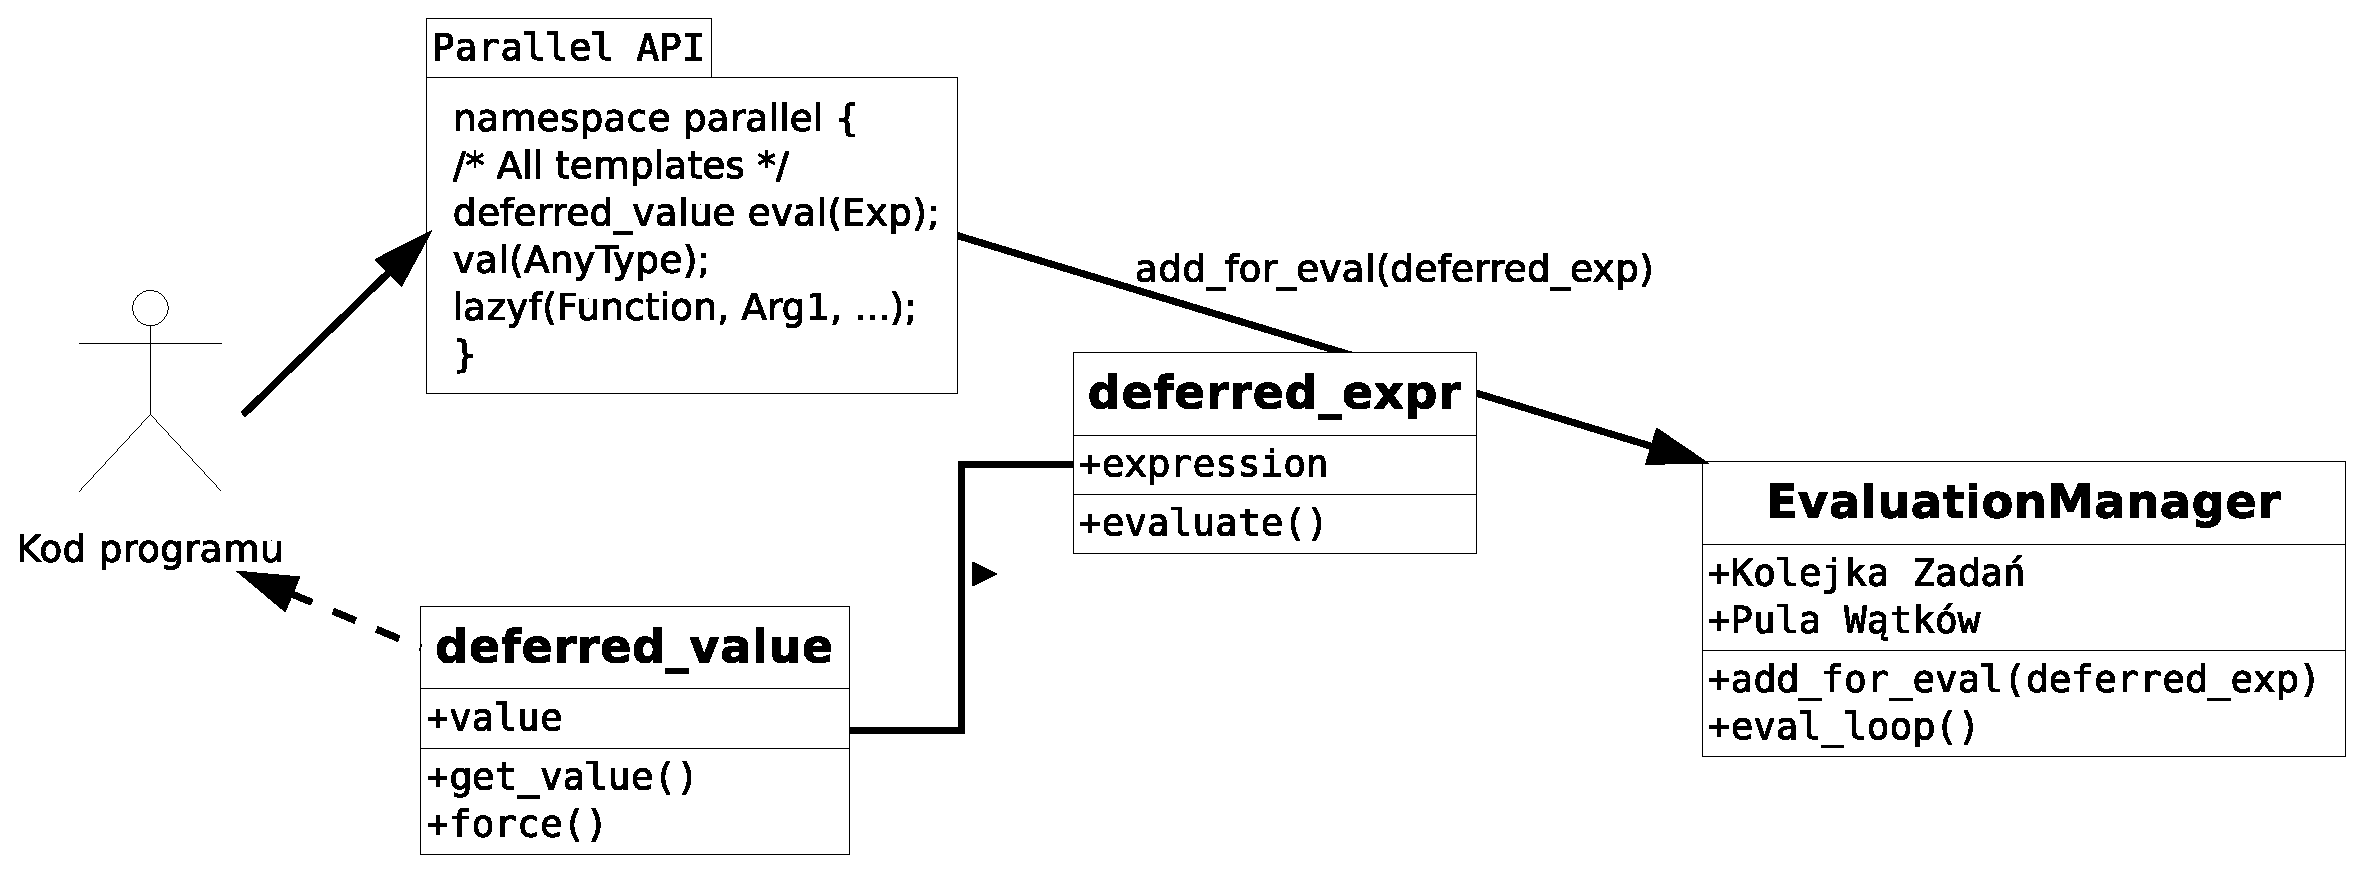
\includegraphics[width=\textwidth]{architecture.eps}
 \caption{Schemat architektury biblioteki Parallel}
\end{figure}

  Na diagramie nie znajduj� si� wszystkie metody zaimplementowane w poszczeg�lnych klasach, a jedynie te niezb�dne do zaprezentowania architektury biblioteki.
  
\subsection{API biblioteki}

  Kod programu komunikuje si� z bibliotek� poprzez API. Oto kr�tkie wyja�nienie znaczenia poszczeg�lnych funkcji z API:
  G��wn� funkcj� z API jest funkcja \feval, kt�rej znaczenie zosta�o opisane w sekcji \nameref{sss:eval}.
  Pozosta�e funkcje maj� zadanie pomocnicze w stosunku do \feval.
  S� niezb�dne do stworzenia wyra�enia, kt�re funkcja \feval mo�e przyj�� do wyliczenia.
  I tak funkcja \verb|val| pozwala przekaza� sw�j argument do wyra�enia przez warto��, \verb|cval| przez warto�� sta��, \verb|ref| przez referencj�, \verb|cref| przez sta�� referencj�.
  Ponadto, w API znajduje sie wzorzec funkcji pozwalaj�cy na uleniwione wywo�ywanie funkcji, \verb|lazyf|.
  Rola i spos�b implementacji tych funkcji s� opisane w sekcji \nameref{s:przekazywanie_wyrazen}.
  
  Nale�y doda�, i� program korzystaj�cy z biblioteki Parallel musi przed rozpocz�ciem zlecania wyra�e� do obliczenia wywo�a� funkcj� \verb|init|
  inicjalizuj�c� bibliotek� i ustalaj�c� liczb� w�tk�w w puli mechanizmu ewaluacji.
  Korzystanie z biblioteki Parallel powinno zako�czy� si� wywo�aniem funkcji \verb|close|, kt�ra zwalnia zasoby zaalokowane przez bibliotek�.
  
\subsection{Operacje wykonywane w kodzie biblioteki Parallel}\label{ss:operacje}

  Odpowiednio stworzone wyra�enie jest przetwarzane przez funkcj� \feval.
  W ciele funkcji z wyra�enia tworzony jest obiekt typu \verb|deferred_expr|, kt�ry reprezentuje zadanie do wykonania.
  Zadanie jest dodawane do kolejki zada� w obiekcie \emgr przy u�yciu metody \verb|add_for_eval|.
  Aparat wykonawczy w postaci instancji typu \emgr zawiera, opr�cz kolejki zada� do wykonania, r�wnie� w�tki, kt�rymi zarz�dza, i kt�re wykonuj� zadania dzia�aj�c w niesko�czonej p�tli w funkcji \verb|eval_loop|.
  
  Ka�dy obiekt typu \verb|deferred_expr| jest po��czony 1-1 z obiektem typu \dval, kt�ry reprezentuje wynik obliczenia wyra�enia.
  Je�li zadanie zdefinowane przez wyra�enie zapami�tane w obiekcie \dexp zostaje wykonane, to wynik (je�li istnieje) zostaje przypisany na pole \verb|m_value| w skojarzonym obiekcie typu \dval.
  
\subsection{Zwr�cenie wyniku}
  
  Wynik jest przekazywany do kodu programu poprzez obiekt typu \verb|deferred_value|, kt�ry jest zwracany jako wynik funkcji \feval.
  Je�li nast�pi wywo�anie pobrania warto�ci z obiektu typu \dval metod� \verb|get_value| lub wymuszenie wyliczenia warto�ci przez metod� \verb|force|, wyliczenie wyra�enia zostaje wymuszone, o ile nie zosta�o ju� wykonane.
  
  
\section{Implementacja przekazywania wyra�e� do wyliczenia}\label{s:przekazywanie_wyrazen}
  
  Jednym z najtrudniejszych zada� podczas fazy implementacji biblioteki Parallel by�o zaprojektowanie przekazywania wyra�e� do wykonania.
  Mechanizm mia� stanowi� wa�n� cz�� API biblioteki, kt�re powinno wspiera� spe�nienie wyznaczonych dla biblioteki cel�w czytelno�ci i intuicyjno�ci.
  Te cele niew�tpliwie by�yby zrealizowane, gdyby mo�liwe by�o przekazywanie wyra�e� w ich standardowej postaci w j�zyku C++.
  Jednak problem stanowi� fakt, i� j�zyk C++ posiada gorliw� semantyk� wyliczania wyra�e�.
  Nale�a�o zatem uleniwi� wyra�enia przekazywane do wyliczenia.
  
  Najbardziej naturalne by�oby u�ycie s�owa kluczowego lub funkcji, kt�ra uleniwia�aby wyra�enie.
  Pierwszy pomys� by� nie do zrealizowania, poniewa� nie mo�na rozszerzy� j�zyka C++ o nowe s�owa kluczowe, a standard C++ nie przewidzia� s�owa kluczowego dla uleniwiania wyra�e�.
  Uleniwienie poprzez u�ycie funkcji mog�oby wygl�da� nast�puj�co:
  \begin{lstlisting}[numbers=none,frame=none]
   make_lazy_expression(4 + fibonacci(20));
  \end{lstlisting}
  Jednak semantyka j�zyka C++ r�wnie� nie pozwala�a na tak� realizacj� uleniwiania wyra�e�, gdy� wyra�enie podane jako argument jest wyliczane przed wywo�aniem funkcji.
  
  Metoda rozwi�zania problemu uleniwiania wyra�e� okaza�a si� by� bardziej skomplikowana i zosta�a zainspirowana przez idiom C++ szablonu wyra�enia,
  kt�ry jako jedna z dobrych praktyk j�zyka C++ zosta� opisany w ksi��ce \textit{More C++ Idioms} \cite{idioms}.
  Implementacja tego szablonu nie by�aby mo�liwa gdyby nie bardzo silny mechanizm szablon�w typ�w i funkcji w j�zyku C++.

\subsection{Szablony w j�zyku C++}

  Ta sekcja nie zawiera podstawowych informacji na temat szablon�w w C++.
  Wprowadzenie do tej tematyki mozna przeczyta� w ksi��ce \cite{c++lang}.
  Moim celem jest pokazanie, dlaczego implementacja przekazywania wyra�e�, tak jak tego dokona�em, by�a mo�liwa.
  
  Szablony s� bardzo silnym mechanizmem. 
  Ciekawostk� jest fakt, �e si�a ekspresyjna szablon�w nie by�a zamierzona przez tw�rc�w w momencie projektowania i mo�liwo�ci, kt�re daj�, zosta�y odkryte p�niej.
  Szablony C++ s� w rzeczywisto�ci pewnym funkcyjnym j�zykiem programowania o ekspresywno�ci rachunku lambda.
  Udowodniono, i� mechanizm szablon�w jest r�wnowa�ny maszynie Turinga (\cite{turingcom}).
  W praktyce oznacza to tyle, �e szablony C++ pozwalaj� dokonywa� dowolnych oblicze� w oparciu o wzorce typ�w.
  Prosz� spojrze� na poni�szy przyk�ad:
  \begin{lstlisting}
template< unsigned n >
struct factorial {
  static const unsigned value = 
    n * factorial<n-1>::value;};
template<>
struct factorial<0> {
  static const unsigned value = 1; };
  \end{lstlisting}
  Wzorzec \verb|factorial| pozwala obliczy� dowolne warto�ci silni w czasie kompilacji
  \footnote{Pewnym ograniczeniem jest limit kompilatora na rekurencyjne konkretyzowanie szablon�w, ale ten limit mo�na zmieni� przy pomocy odpowiednich opcji} i korzysta� z nich w czasie sta�ym podczas wykonania programu.
  Obliczenie odbywa si� rekurencyjnie, warunkiem ko�cz�cym rekurencj� jest \verb|factorial<0>|, kt�re jest specjalizacj� szablonu \verb|factorial|.
  
  
\subsection{Idiom C++ szablonu wyra�enia}

  Intuicyjnie rzecz ujmuj�c, idiom szablonu wyra�enia polega na opisaniu wyra�enia przy pomocy konkretyzacji pewnego szablonu typu.
  Ten typ nie jest nigdy zapisywany w postaci jawnej w programie, gdy� mo�na przypuszcza�, �e sk�adnia szablonu typu by�aby wtedy bardzo nieczytelna.
  Zamiast tego szablon typu jest tworzony w wyniku oblicze� na typach udost�pnianych przez mechanizm rozwijania szablon�w w j�zyku C++.
  Idiom szablonu wyra�enia wykorzystuje inny idiom Rekurencyjnego Sk�adania Typ�w (z ang. Recursive Type Composition). 
  Polega on na tym, �e szablon typu zawiera pola, kt�rych typem jest jest konkretyzjacja tego samego szablonu typ�w.
  W tym przypadku szablon wyra�enia mo�e zawiera� pola, kt�re s� szablonem wyra�enia.
  W ten spos�b powstaje reprezentacja wyra�enie w postaci drzewa typ�w. 
  Taka konstrukcja nazywana jest Abstrakcyjnym Drzewem Syntaktycznym (z ang. Abstract Syntax Tree - AST).
  W li�ciach drzewa znajduj� si� terminale wyra�enia, czyli warto�ci, referencje b�d� wska�niki.
  Natomiast w w�z�ach po�rednich reprezentowane s� operatory u�yte w wyra�eniu, kt�re jako pola posiadaj� szablony wyra�enia, b�d�ce argumentami operatora.
  Ka�demu operatorowi odpowiada reprezentuj�cy go szablon typu, z odpowiednio zaimplementowan� funkcj� aplikuj�c� operator, w momencie, gdy szablon wyra�enia jest wyliczany.
  
  Zaprezentuj� ide� szablonu wyra�enia na przyk�adzie, w kt�rym jedyn� dozwolon� operacj� b�dzie dodawanie liczb ca�kowitych lub zmiennoprzecinkowych.
\begin{lstlisting}
/*** TYPY ODPOWIEDZIALNE ZA BUDOW� DRZEWA AST ***/

template <typename T> struct Exp;

template <typename T>
struct Term : Exp<Term<T> >
{
  Term(T v) : val(v){}
  const T val;
};

/* Definicje wez��w reprezentuj�cych operatory */

template <typename T1, typename T2>
struct Sum : Exp<Sum<T1, T2> >
{
  Sum (T1 l, T2 r) : lhs(l), rhs(r) {}
  const T1 lhs;
  const T2 rhs;
};

template <typename T1, typename T2>
struct Mul: Exp<Mul<T1, T2> >
{
  Mul(T1 l, T2 r) : lhs(l), rhs(r) {}
  const T1 lhs;
  const T2 rhs;
};

/* Wzorzec Infer s�u�y do obliczania typu wynikowego wyra�enia */

template <typename E> 
struct Infer {
  typedef E type ; 
};

template <typename T>
struct Infer<Term<T> >
{
  typedef T type;
};

/* Wnioskowanie dla sumy zgodnie z semantyk� j�zyka C++ */

template < >
struct Infer< Sum<double,double> > 
{ 
  typedef double type; 
};

template < >
struct Infer< Sum<double,int> > 
{
  typedef double type;
};

template < > 
struct Infer< Sum<int,double> > 
{
  typedef double type; 
};

template < > 
struct Infer< Sum<int,int> > 
{ 
  typedef int    type;
};

/* Typ(T1 + T2) to typ sumy(typ(T1),typ(T2)) */
template <typename T1, typename T2> 
struct Infer < Sum<T1,T2> > {
  typename Infer<T1>::type typedef T1T ;
  typename Infer<T2>::type typedef T2T ;
  typename Infer<Sum<T1T,T2T> >::type typedef type;
} ;

/* Wnioskowanie o typach dla wzorca Mul jest analogiczne */

/* Wzorzec Exp umo�liwia unikni�cie definicji operator�w
 * w ka�dym typie reprezentujacym weze� po�redni w drzewie AST */
 
template <typename T>
struct Exp
{
  template <typename U>
  inline Sum<T,U> operator + (U u) 
  { 
    /* static_cast jest potrzebny i prawid�owy, 
     * poniewa� Exp jedynie obudowuje typ T */
    return Sum<T,U>(static_cast<T>(*this), u); 
  }
  
  template <typename U>
  inline Mul<T,U> operator * (U u)
  {
    return Mul<T,U>(static_cast<T>(*this), u);
  }
};

template <typename T, typename U>
Sum<T,U> operator + (T t, Exp<U> u)
{
  return Sum<T,U>(t, static_cast<U>(u));
}

template <typename T, typename U>
Mul<T,U> operator * (T t, Exp<U> u)
{
  return Mul<T,U>(t, static_cast<U>(u));
}

/*** DEFINICJE FUNKCJI EWALUUJ�CYCH DRZEWA AST ***/

inline template <typename T>
Infer<T>::type eval(Exp<T> exp)
{
  return eval(static_cast<T>(exp));
}

inline template <typename T>
Infer<Term<T> >::type eval(Term<T> term)
{
  return term.val;
}

inline template <typename T1, typename T2>
Infer<Sum<T1, T2> >::type eval(Sum<T1, T2> sum)
{
  return eval(sum.lhs) + eval(sum.rhs);
}

inline template <typename T1, typename T2>
Infer<Mul<T1, T2> >::type eval(Mul<T1, T2> mul)
{
  return eval(mul.lhs) + eval(sum.rhs);
}

/* Potrzebna jest tak�e definicja int eval (int) 
 * oraz double eval(double), poniewa� nie ma wymogu,
 * aby zawsze te typy proste by�y obudowane w Term. */
 
inline int eval(int i) {return i;}
inline double eval(double d) {return d;}
\end{lstlisting}

  Wzorzec \verb|Term| (linie 6-11) umo�liwia oznaczenie dowolnej warto�ci jako li�cia w drzewie reprezentujacym szablon wyra�enia.  
  Teoretycznie wszystkie warto�ci powinny byc oznaczone w ten spos�b.
  Jednak jak sie p�niej dowiemy identyczne dzia�anie mo�na uzyska� oznaczaj�c tylko niekt�re z warto�ci.
  
  Wzorce \verb|Sum| oraz \verb|Mul| reprezentuj� wez�y po�rednie w drzewie AST (linie 15-29).
  Ich pierwszy i drugi parametr reprezentuj� odpowiednie podwyra�enia, b�d�ce argumentami operatora binarnego.
  Najciekawszym zabiegiem u�ytym w ich definicji jest podanie definicji tego� samego wzorca jako argumentu wzorca Exp, b�d�cego klas� bazow� wzorc�w operator�w.
  Ma to miejsce przyk�adowo w tym fragmencie kodu: \verb|struct Sum : Exp<Sum<T1, T2> >| i jest w pe�ni dozwolone przez sk�adni� j�zyka.
  Dzi�ki takiemu zabiegowi mo�na poda� implementacj� operator�w tylko we wzorcu \verb|Exp|, a nie jest to konieczne we wszystkich innych wzorcach w�z��w po�rednich.
  \verb|Sum<T1, T2>| dziedziczy metody przedefiniuj�ce operatory, z tym, �e te definicje s� dopasowane do \verb|Sum<T1, T2>|, poniewa� s� parametryzowane tym typem.
  
  Kolejna cz�� przyk�adu (linie 33-78) to definicja wzorca \verb|Infer|, kt�ry oblicza typ wynikowy wyliczenia wyra�enia, b�dzie on potrzebny do definicji funkcji ewaluuj�cych wyra�enie.
  Wykorzystywany jest tutaj mechanizm specjalizacji wzorc�w, kt�ry pozwala okre�li� typ wynikowy wyra�enia w zale�no�ci od postaci wzorca.
  Og�lnie, podczas definicji wnioskowania o typach nale�y pami�ta� o uwzgl�dnieniu wszystkich istotnych specjalizacji wzorca, czyli dla w�z��w po�rednich jak \verb|Term|, \verb|Sum|, \verb|Mul|
  oraz wszystkich mo�liwych typ�w, kt�re mog� wystapi� w w�z�ach po�rednich.
  Jak wida� implementacja szablonu wzorca wnioskuj�cego o typie wynikowym wyra�enia jest bardzo d�uga i czasoch�onna (do tego stopnia, �e pomin��em cz�� po�wi�con� wnioskowaniu typu dla
  wzorca \verb|Mul|, gdy� jest ona analogiczna jak cz�� dotycz�ca wzorca \verb|Sum|.
  Na koniec sekcji kodu, kt�ra tworzy AST (linie 83-99) znajduje si� definicja wzorca \verb|Exp|, kt�ry przeci��a operatory dla szablonu wyra�enia.
  
  Kolejna sekcja kodu przyk�adu (linie od 103 do 132) definiuje funkcj� \feval, kt�ra s�u�y do obliczania warto�ci szablonu wyra�enia.
  Funkcja \feval przyjmuje jako argument szablon wyra�enia (albo warto�� prost� int lub double), a nast�pnie oblicza jego warto�� zgodnie z semantyk� j�zyka C++.
  Typ zwracany przez \feval jest obliczany przy pomocy wzorca \verb|Infer|.
  
\subsubsection{Szablon wyra�enia w dzia�aniu}
  Zrozumienie kodu szablonu wyra�enia przedstawionego powy�ej b�dzie �atwiejsze po przeanalizowaniu przyk�ad�w jego dzia�ania.
  We�my najprostszy mo�liwy przyk�ad:
  \begin{lstlisting}[numbers=none, frame=none]
   Term(4) + Term(5);
  \end{lstlisting}
  Wyra�enie dodaje dwie liczby ca�kowitych.
  Szablon wyra�enia, kt�ry je reprezentuje, zostanie stworzony w wyniku oblicze� na typach i b�dzie wygl�da� nast�puj�co:
  \begin{lstlisting}[numbers=none, frame=none]
   Sum<Term<int>,Term<int> >
  \end{lstlisting}
  Ju� na bazie tego prostego przyk�adu nasuwa si� kilka ciekawych kwestii do om�wienia.
  
  Po pierwsze mo�na si� zastanowi�, po co sk�adania jest tak ``przegadana'' oraz czy potrzebne jest pisanie \verb|Term| przy ka�dej warto�ci przekazywanej do wyra�enia.
  Wiadomo na pewno, �e co najmniej jedna warto�� musi by� oznaczona jako terminal szablonu wyra�enia.
  W przeciwnym przypadku, by�oby to zwyk�e wyra�enie C++, �adna z warto�ci nie zosta�aby uleniwiona i zosta�oby obliczone gorliwie.
  
  Zastan�wmy si�, czy poni�sze wyra�enie jest poprawne sk�adniowo i je�li tak, to jaki b�dzie szablon typu, kt�ry powstanie.
  \begin{lstlisting}[numbers=none, frame=none]
   Term(4) + 5;
  \end{lstlisting}
  W tym wyra�eniu mamy do czynienia z operacj� dodawania warto�ci typu \verb|Term<int>| oraz typu \verb|int|.
  Poniewa� \verb|Term<int>| dziedziczy operator dodawania z \verb|Exp<Term<int> >| to zostanie wywo�any operator dodawania zdefinowany w linii 87 przyk�adu.
  Warto zauwa�y�, �e typ prawego argumentu przeci��onego operatora nie jest w �aden spos�b ograniczony, wi�c zastosowanie typu int jest poprawne.
  W zwi�zku z tym wynikiem budowy drzewa tego wyra�enia b�dzie \verb|Sum<Term<int>, int>|.
  Pokazuje to, �e szablon wyra�enia zostanie zbudowany poprawnie r�wnie� wtedy, gdy nie wszystkie warto�ci zostan� oznaczone jako terminale.
  Jednak�e, cz�� warto�ci, a co najmniej jedna musi zosta� oznaczona, gdy� inaczej budowa szablonu wyra�enia nie zostanie zapocz�tkowana i wyra�enie nie zostanie uleniwione, a obliczy si� normalnie.
  
  Wa�nym faktem jest to, �e budowa drzewa AST ma miejsce w czasie kompilacji, wi�c budowanie szablon�w wyra�e� nie nak�ada narzut�w na czas wykonania programu.
  Natomiast narzuty podczas ewaluacji uleniwionego wyra�enia zale�� od tego w jakim stopniu kompilator zoptymalizowa� wywo�ania funkcji \feval wyliczaj�cej warto�� wyra�enia poprzez jej rekurencyjne rozwini�cie w miejscu wykonania.
  W najgorszym przypadku b�dzie mia�o miejsce jedno wywo�anie funkcji dla ka�dego w�z�a po�redniego.
  
  Teraz na bardziej zaawansowanym przyk�adzie zbadamy jakie s� zasady decyduj�ce o tym, kiedy dodanie oznaczenia \verb|Term| jest wymagane, aby uleniwienie wyra�enia dzia�a�o zgodnie z �yczeniem programisty.
  Do tej analizy pos�u�� dwa przyk�ady uleniwionych wyra�e�:
  \begin{lstlisting}[frame=none, numbers=none]
   4 + 5 * Term(6); /* (1) */
   
   Term(4) + 5 * 6; /* (2) */
  \end{lstlisting}
  Nale�y mie� �wiadomo��, �e du�� rol� w procesie budowy drzewa AST odgrywaj� w�asno�ci operator�w.
  Liczba ich argument�w, priorytety i kierunek wi�zania decyduj� o postaci drzewa, a tym samym o uleniwieniu wyra�enia.
  
  W pierwszym wyra�eniu najpierw kompilator zajmie si� podwyra�eniem \verb|5 * Term(6)|, kt�re da w rezultacie \verb|Mul<int, Term<int> >|.
  Warto odnotowa�, �e tym razem tylko prawy argument operatora binernego by� typem szablonu wyra�enia, wi�c zosta� u�yty operator zdefinowany w linii 108 przyk�adu.
  W nastepnej kolejno�ci nast�pi dodawanie 4 oraz wyra�enia typu \verb|Mul<int, Term<int> >|, co da w wyniku kolejny bardziej rozbudowany szablon wyra�enia \verb|Sum<int, Mul<int, Term<int> > >|.
  Uda�o si� pokaza�, �e pierwsze z analizowanych wyra�e� zachowa si� zgodnie z intencj� programisty, to znaczy ca�e wyra�enie zostanie uleniwione.
  
  Analogicznie badamy zachowanie wyra�enia drugiego.
  Na pocz�tku spostrzegamy, �e najpierw dojdzie do obliczenia podwyra�enia \verb|5 * 6|. 
  Zatem ewaluacja odb�dzie si� gorliwie, poniewa� budowa szablonu wyra�enia nie zosta�a zapocz�tkowana, mamy tu do czynienia ze zwyk�ym mno�eniem.
  W nast�pnym kroku odb�dzie si� dodawanie \verb|Term(4)| i wyniku \verb|5 * 6|, czyli \verb|30|, czego konsekwencj� b�dzie stworzenie szablonu wyra�enia \verb|Sum<Term<int>, int>|.
  To nie jest to czego oczekiwali�my, gdy� za�o�yli�my, �e chcemy uleniwi� ca�e wyra�enie, a zasz�o to jedynie dla jego cz�ci.
  
  Wnioskiem z powy�szej analizy jest regu�a propagacji leniwo�ci w czasie budowania szablonu wyra�enia.
  Propagowanie zachodzi od warto�ci oznaczonej jako terminal w g�r� drzewa.
  St�d ka�dy operator na �cie�ce pomi�dzy uleniwionym terminalem, a korzeniem drzewa (w��cznie) b�dzie uleniwiony, czyli nie b�dzie wywo�any od razu, 
  a zostanie zakodowany w strukturze szablonu wyra�enia i wywo�any, gdy nast�pi wymuszenie obliczenia wyra�enia.
  W szczeg�lno�ci, pisz�c kod tworz�cy szablony wyra�enia w oparciu o przedstawiony przyk�ad nale�y mie� na uwadze to, �e tworzenie drzew AST przez kompilator nie jest jednoznaczne,
  poniewa� kompilator mo�e w przypadku wyst�pienia obok siebie operator�w o identycznym priorytecie stworzy� r�ne drzewa AST.
  Przyk�adem jest wyra�enie \verb|4 + 5 + 6|.
  
\subsection{Praktyczna implementacja szablonu wyra�enia -- Boost Proto}

  Przedstawiony powy�ej spos�b da si� uog�lni� dla dowolnego wyra�enia w j�zyku C++.
  To znaczy, �e stworzenie dowolnego leniwego wyra�enia jest mo�liwe, do czego d��y�em podczas tworzenia implementacji Parallel.
  Jednak�e napisanie takiej biblioteki od podstaw wykracza�o poza ramy tej pracy magisterskiej.
  Dlatego si�gn��em po rozwi�zania ju� istniej�ce, publicznie dostepne i sprawdzone.
  W celu implementacji uleniwionych wyra�e� metod� szablon�w wyra�e� wybra�em bibliotek� Boost Proto.
  
  Boost Proto jest bibliotek� s�u��c� do tworzenia Wbudowanych J�zyk�w Domenowych (z ang. Domain Specific Embedded Language) w j�zyku C++. 
  Zawiera narz�dzia do tworzenia, sprawdzania typ�w, przetwarzania oraz ewaluacji szablon�w wyra�e�. Proto zapewnia:
  \begin{itemize}
   \item Szablony wyra�e� w postaci AST
   \item Mechanizm modyfikacji zachowania wyra�e�
   \item Przeci��anie operator�w dla budowy AST z wyra�enia
   \item Narz�dzia do definiowania gramatyki wyra�e�
   \item Rozszerzalny mechanizm wyliczenia szablonu wyra�enia
   \item Rozszerzalny zestaw operacji przetwarzania szablon�w wyra�e�
  \end{itemize}

  Biblioteka Boost Proto zosta�a wykorzystana do implementacji nast�puj�cych komponent�w biblioteki Parallel:
  \begin{itemize}
   \item Funkcje do oznaczania terminali:
   \begin{itemize}
    \item \verb|val| -- funkcja przekazuj�ca terminal do wyra�enia przez warto��
    \item \verb|cval| -- funkcja przekazuj�ca terminal do wyra�enie przez warto�� sta��
    \item \verb|ref| -- funkcja przekazuj�ca terminal do wyra�enia przez referencj�
    \item \verb|cref| -- funkcja przekazuj�ca terminal do wyra�enia przez referencj� sta��
   \end{itemize}
   \item \verb|lazyf| -- funkcja s�u��ca do tworzenia uleniwionego wywo�ania funkcji
   \item \verb|deferred_expr| -- szablon typu przechowuj�cego uleniwione wyra�enia i zarz�dzaj�cego jego wyliczeniem
  \end{itemize}
  
  Biblioteka Parallel korzysta z Boost Proto do tworzenia szablon�w wyra�e� w postaci AST, r�wnie� przy pomocy mechanizmu przeci��ania operator�w, dzi�ki czemu budowa AST jest uproszczona.
  Ponadto ewaluacja odbywa si� przy pomocy dostarczonej przez Boost Proto funkcji \verb|proto::eval| z domy�lnym zachowaniem.
  Zasada dzia�ania Boost Proto jest analogiczna do dzia�ania przyk�adu pokazanego powy�ej.

\subsection{Alternatywne rozwi�zanie}

  Do wyboru by�a r�wnie� inna mo�liwo�� realizacji przekazywania wyra�enia ni� forma uleniwiona opisana to powy�ej.
  Podobny efekt mo�na uzyska� stosuj�c obiekty funkcyjne, kt�re reprezentowa�yby dane wyra�enie.
  Istnieje jednak istotny pow�d, dla kt�rego zosta�o wybrane pierwsze z przedstawionych rozwi�za�.
  Leniwe wyra�enia maj� bardziej intuicyjn� sk�adni�, natomiast tworzenie odpowiednich obiekt�w funkcyjnych wymaga znajomo�ci stosownych bibliotek.
  Przyk�adami s� Boost.Lambda, Boost.Function i Boost.Bind, jednak�e pomimo tego, �e s� to jedne z najlepszych bibliotek w swojej klasie, w przypadku pisania rozbudowanego wyra�enia ich sk�adnia jest zdecydowanie nieintuicyjna.
  Szczeg�lnie problematyczny jest zapis zagnie�d�onych funkcji, w tym operator�w.
  Nast�puj�cy kawa�ek kodu nie nale�y do czytelnych:
\begin{verbatim}
  bind(f, bind(operator+,4, (bind(operator*, 5, 6)))); //f(4 + 5 * 6)
\end{verbatim}
  Zamiast bardziej intuicyjnego:
\begin{verbatim}
  lazyf(val(4) + val(5) * val(6));
\end{verbatim}
  Tak naprawd� wystarczy�oby
\begin{verbatim}
 lazyf(f, 4 + val(5)*6);
\end{verbatim}
  gdy� \verb|val(5)| wprowadzi�oby leniwo�� na najni�szym poziomie w drzewie wyra�enia, kt�ra nast�pnie propagowa�aby si� w g�r� drzewa.

  Dlatego, ze wzgl�du na znacznie bardziej intuicyjn� sk�adni�, wybrano leniwe wyra�enia do realizacji przekazywania oblicze� do wykonania r�wnoleg�ego.

\section{Implementacja mechanizmu ewaluacji}\label{s:ewaluacja}

  Zarys mechanizmu ewaluacji zosta� przedstawiony w sekcji \nameref{ss:wykonywanie}.
  G��wn� funkcj� mechanizmu ewaluacji jest pobieranie zada� (wyra�e� do obliczenia) zlecanych przez kod programu i ich ewaluacja.
  Do implementacji tej cz�ci biblioteki wykorzystano wzorzec projektowy puli w�tk�w oraz kolejki zada�.
  G��wn� klas� tej cz�ci biblioteki jest \verb|evaluation_mgr| (od ang. evaluation manager -- mened�er ewaluacji), kt�ra jest singletonem i zarz�dza ca�o�ci� procesu wykonywania zada�.
  
\subsection{Zadania w bibliotece Parallel}

  Zadaniem w kontek�cie biblioteki Parallel nazywam uleniwione wyra�enie, kt�re zosta�o przekazane bibliotece do obliczenia.
  Zadanie jest reprezentowane przez konkretyzacj� wzorca typu \verb|deferred_expr| (od ang. deferred expression -- wyra�enie odroczone).
  Jedyny konstruktor publiczny tego wzorca przyjmuje jako argument szablon wyra�enia, taki jaki zosta� opisany w sekcji \nameref{s:przekazywanie_wyrazen}.
  Szablon wyra�enia jest przechowywany jako jedno z p�l \verb|deferred_expr| i poddawany ewaluacji po wywo�aniu metody \verb|evaluate|.
  Pozosta�e pola i metody \verb|deferred_expr| s�u�a kontrolowaniu wyliczenia wyra�enia oraz przekazywaniem wyniku do skojarzonego obiektu typu \verb|deferred_value|
  \footnote{Zgodnie z opisem z \nameref{ss:operacje} obiekt \dexp jest skojarzony 1-1 z obiektem \dval.}.
  
\subsection{Pula w�tk�w}

  Wzorzec puli w�tk�w zosta� wybrany ze wzgl�du na efektywno��.
  Dzi�ki takiej implementacji unika si� tworzenia w�tku dla ka�dego zadania do wykonania, co jest operacj� dosy� drog� i warto zadba�, aby nie by�a wykonywana zbyt cz�sto.
  Ka�dy z w�tk�w dzia�a w niesko�czonej p�tli w funkcji \verb|eval_loop|, w kt�rej w�tek pr�buje pobra� zadanie do wykonania z kolejki zada�, a je�li nie jest ono dost�pne to czeka na zmiennej warunkowej.
  Do implementacji zosta�a wykorzystana biblioteka Boost.Threads.
  
  Pula w�tk�w pozwala unikn�� innego problemu zwi�zanego z tworzeniem w�tku dla ka�dego zadania.
  W przypadku gdyby pojawi�o si� zbyt wiele zada� jednocze�nie liczba w�tk�w mog�aby wzrosn�� do takiej liczby, �e wydajno�� programu znacznie by spad�a z powodu cz�stego prze��czania kontekstu pomi�dzy r�nymi w�tkami.
  Pula w�tk�w pozwala ustali� maksymaln� liczb� w�tk�w, co przedziwdzia�a przeci��eniu systemu.
  Obecnie liczba w�tk�w jest ustalana przez programist�, nic nie stoi na przeszkodzie, aby w przysz�o�ci liczba w�tk�w by�a dobierana automatycznie w zale�no�ci od wydajno�ci systemu b�d� innych parametr�w.
  
\subsection{Kolejka zada�}

  Kolejka zada� jest standardow� kolejk� FIFO przechowuj�c� obiekty \dexp.
  Poniewa� jednocze�nie kod programu lub ka�dy z w�tk�w z puli przechowywanej w \verb|evaluation_mgr| mo�e chcie� skorzysta� z kolejki, dost�p do niej jest chroniony sekcj� krytyczn�.
  Dodawanie zada� do kolejki odbywa si� w ciele funkcji \feval przy u�yciu funkcji \verb|add_for_eval|.

\subsection{Procedura ewaluacji}

  Procedura ewaluacji z punktu widzenia mechanizmu ewaluacji wygl�da bardzo prosto.
  W�tek-robotnik pobrawszy zadanie wywo�uje jego metod� \verb|evaluate|.
  To skutkuje wyliczeniem wyra�enia, a je�li typ wynikowy wyra�enia jest inny ni� \verb|void| to warto�� zostaje przekazana do skojarzonego obiektu \dval.
  Po wyliczeniu wyra�enia obiekt \dexp jest niszczony, gdy� nie jest ju� potrzebny.
  
  Ten obraz komplikuje si�, gdy rozwa�ymy pewien bardzo istotny scenariusz.
  Ot� nie ma problemu je�li, w�tki-robotnicy dokonuj� ewaluacji zada� z kolejki odpowiednio szybko.
  Jednak, gdy d�ugo�� kolejki wzro�nie mo�e doj�� do tego, �e w�tek programu, kt�ry zleci� wyliczenie wyra�enia oczekuj�cego w kolejce, b�dzie potrzebowa� jego wyniku.
  Wtedy nast�pi pr�ba pobrania warto�ci z obiektu \dval, kt�ry jeszcze nie otrzyma� obliczonej warto�ci.
  To oznacza, �e w�tek programu musia�by zawiesi� wykonywanie i poczeka�, a� warto�� zostanie obliczona.
  
  Gdy w�tek programu oczekuje na wyra�enie, kt�rego ewaluacja ju� si� rozpocz�a, to nie ma innego wyj�cia ni� poczekanie na doko�czenie oblicze�.
  Jednak, gdy zadanie, na kt�re program oczekuje, jeszcze nie zosta�o pobrane do wykonania dosz�oby do absurdalnej sytuacji, 
  poniewa� program zawiesi�by si� i czeka�by na wykonanie zadania, podczas gdy sam m�g�by wykona� potrzebne obliczenia.
  Odpowienio zaimplementowana procedura ewaluacji uwzgl�dnia ten problem.
  
  W analogicznej sytuacji w�tek programu, gdy zorientuje si�, �e wyra�enie nie zosta�o obliczone sam dokona ewaluacji.
  Zostanie wywo�ana ta sama procedura \verb|evaluate|, kt�r� wywo�uj� w�tki-robotnicy.
  Mo�e to skutkowa� zdublowanym wyliczeniem wyra�enia, w przypadku, gdy zar�wno w�tek programu, jak i jeden z w�tk�w-robotnik�w obliczyliby wyra�enie.
  Taka sytuacja by�aby niedopuszczalna, poniewa� wykonywanie wyra�enia w C++ nie jest idempotentne z powodu efekt�w ubocznych.
  
  Najbardziej standardowym rozwi�zaniem by�oby umieszczenie w ka�dym obiekcie \dexp flagi wraz mutexem j� chroni�cym w celu zapobie�enia podw�jnej ewaluacji wyra�enia.
  Jednak�e umieszczenie mutex-a w ka�dym obiekcie ma pewien narzut pami�ciowy i wydajno�ciowy.
  
  Istnieje lepsze rozwi�zanie tego problemu wykorzystuj�ce funkcj� z biblioteki Boost Threads \verb|call_once| gwarantuj�c� jednokrotne wywo�anie pewnej instrukcji.
  Przekazanie tej funkcji zmiennej typu \verb|once_flag| wraz z funkcj� do wykonania (w tym przypadku funkcj� \verb|deferred_expr::evaluate|) sprawia, �e dla danej flagi funkcja wykona si� tylko raz.
  Wywo�anie \verb|call_once| z ju� raz wykorzystan� flag� \verb|once_flag| zako�czy si� natychmiast bez wywo�ania przekazanej funkcji.
  Poniewa� typ \verb|once_flag| ma niewielki rozmiar (na wi�kszo�ci platform jest to typ \verb|long|) to umieszczenie go jako pola ka�dego obiektu \dexp dodaje mniejszy narzut pami�ciowy ni� stosowanie mutex�w.
  
  Innym wa�nym aspektem procedury ewaluacji odroczonego wyra�enia jest obs�uga wyj�tk�w.
  Zgodnie z koncepcj� biblioteki wyj�tki, kt�re wyst�pi� podczas ewaluacji wyra�enia (w ciele funkcji \verb|evaluate| s� wywo�ywane, a nast�pnie przekazywane do obiektu \dval zamiast wyniku.
  Dzi�ki temu wyj�tek b�dzie m�g� zosta� przekazany z obiektu \dval do g��wnego w�tku programu.
  
\subsection{Ograniczenia mechanizmu ewaluacji}

  W zwi�zku ze sposobem przekazywania wyra�e� do obliczenia, mo�liwo�ci projektowania mechanizmu ewaluacji by�y do�� powa�nie ograniczone.
  W og�lno�ci mogliby�my wyobrazi� sobie sytuacj�, w kt�rej wyra�enie z programu dzia�aj�cego na jednym komputerze by�oby przekazywane do wyliczenia do innych program�w lub nawet do innych komputer�w, w celu wi�kszego rozproszenia i jeszcze lepszego zr�wnoleglenia wykonania programu.
  W przypadku biblioteki parallel wyst�pi�o kilka ogranicze�, kt�re uniemo�liwi�y zaprojektowanie og�lniejszego mechanizmu oblicze�.
  
  Migracja kodu (taka jak zosta�� opisana w ksi��ce \cite{dissys}) nie jest wspierana przez j�zyk C++, poniewa� kod kompilowany jest do natywnego kodu maszynowego, a nie kodu po�redniego.
  Nie ma mo�liwo�ci zserializowania fragmentu oblicze� i przes�ania do wykonania na innym komputerze, o nieznanej architekturze.
  W przeciwie�stwie do j�zyka C++ to jest wykonalne w j�zyku Java.
  
  Alternatyw� dla wsparcia j�zyka dla migracji kodu jest rozszerzenie biblioteki o narz�dzia automatycznie generuj�ce kod dla klienta (programu zlecaj�cego obliczenia) i serwera (programu wykonuj�cego obliczenia).
  To przypomina metod� tworzenia RPC i rodzi szereg innych problem�w r�wnie� opisanych w \cite{dissys}.
  Implementacja takiego modelu prowadzenia oblicze� w bibliotece Parallel wykracza�aby poza ramy nakre�lonej pracy oraz mog�aby ograniczy� u�yteczno�� biblioteki ze wzgl�du na bardziej skomplikowany proces programowania i kompilacji.
  
  Kolejne z ogranicze� jest zwi�zane z obecno�ci� w wyra�eniu przekazywanym do obliczenia warto�ci typu referencje lub wska�niki, kt�re s� �ci�le zale�ne od przestrzeni adresowej programu. 
  Przes�anie ich nawet do innego programu na tym samym komputerze wymaga�oby wykorzystania specjalnej procedury, gdy� proste przekazanie warto�ci tego typu powodowa�oby b��dy w dost�pie do pami�ci.
  Obej�cie tego problemu oferuje mechanizm pami�ci wsp�dzielonej, ale powoduje znaczny narzut zwi�zany z dost�pnem do tego rodzaju pami�ci.
 
  Wymienione powy�ej ograniczenia uzasadniaj� podj�cie decyzji o przyj�ciu dla biblioteki Parallel mechanizmu ewaluacji wyra�e� opartego o w�tki.

\section{Implementacja zwracania wyniku oblicze�}
  
  Mo�liwo�� zwracania wynik�w z oblicze� wykonywanych przez inny w�tek jest jedn� z najwa�niejszych cech przemawiaj�cych na korzy�� biblioteki Parallel w por�wnaniu do standardowych bibliotek oferuj�cych wielow�tkowo��.
  Najwa�niejszym elementem procesu zwracania wynik�w przez bibliotek� Parallel jest wzorzec typu \dval parametryzowany typem wyniku wyra�enia.
  Obiekty tego typu s� po�rednikami, kt�re przekazuj� informacje z kodu biblioteki do kodu programu.
  
\subsection{Podstawowe w�a�ciwo�ci wzorca typu \dval}

\subsubsection{Przekazanie warto�ci}

  Obiekt typu \dval po utworzeniu i zwr�ceniu przez funkcj� \feval posiadaj� warto�� nieokre�lon�.
  Dopiero po obliczeniu wyra�enia zapami�tanego w skojarzonym obiekcie \dexp, otrzymana warto�� jest przekazywana do obiektu \dval w celu jej zapami�tania.
  Poniewa� obiekt \dexp jako jedyny ma prawo dokonania takiego przypisania, nie jest konieczna ochrona przed wsp�bie�nym zapisem do obiektu \dval.
  
\subsubsection{Wymuszenie wyliczenia wyra�enia}

  Obiekt typu \dval pozwala na kontrolowanie w pewnym stopniu wyliczenia wyra�enia przez programist�.
  Mianowicie, wywo�anie metody \verb|force| powoduje wymuszenie wyliczenia wyra�enia.
  Zatem programista w razie takiej potrzeby mo�e uzyska� pewno��, �e ewaluacja wyra�enia zosta�a zako�czona.
  Ponadto, do wymuszenia wyliczenia wyra�enia zawsze dochodzi wtedy, gdy pobierana jest warto�� wyra�enia.
 
\subsubsection{Pobranie warto�ci}

  Obiekt typu \dval pozwala na pobranie warto�ci poprzez wywo�anie metody \verb|get_value| lub te� niejawnie, poniewa� poprzez operator konwersji do typu, kt�ry reprezentuje.
  Zatem taki ci�g instrukcji:
  \begin{lstlisting}[numbers=none, frame=none]
   deferred_value<int> d = parallel::eval(parallel::val(4) + 5);
   /* ... */
   int c = d + 42;
  \end{lstlisting}
  jest poprawny syntaktycznie.
  Zatem obiektu typu wzorcowego \dval mo�na u�y� w ka�dym miejscu, gdzie dozwolone jest u�ycie typu wynikowego wyra�enia.
  Skutkuje to wywo�aniem operatora konwersji i pobraniem warto�ci.
 
  Alternatywnym sposobem definicji wzorca \dval by�o nie umieszczanie w jego interfejsie operatora konwersji.
  Uniemo�liwi�oby to stosowanie obiekt�w typu \dval w miejsce typu wynikowego wyra�enia, co sprawi�oby, �e pobieranie warto�ci sta�oby si� operacj� zawsze wywo�ywan� jawnie przez programist�.
  W trakcie projektowania interfejsu biblioteki podj�to decyzj� o umieszczeniu operatora konwersji, poniewa� czyni to sk�adni� bardziej naturaln�.
  Ponadto u�ywanie obiekt�w typu \dval w wyra�eniach bez jawnego pobierania warto�ci ma bardzo istotne znaczenie dla pe�nego wykorzystania funkcji przeci��aj�cych operatory dla wzorca typu \dval.
  Ta kwestia zostanie wyja�niona w nast�pnej sekcji.
  
\subsection{Przeci���nie operator�w szablonu typu \dval}

\subsubsection{Motywacja dla przeci��ania operator�w}

  Mo�na wyobrazi� sobie scenariusz, w kt�rym chc�c skorzysta� z warto�ci przechowywanej w zmiennej typu \dval, 
  programista zawsze wywo�ywa�by jawn� metod� pobrania warto�ci b�d� stosowa�by niejawn� metod�, przy u�yciu operatora konwersji.
  Wygl�da�oby to w kodzie w spos�b nast�puj�cy.
  Wersja z jawnym pobraniem warto�ci:
  \begin{lstlisting}[numbers=none, frame=none]
    deferred_value<int> d = parallel::eval(parallel::val(4) + 5);
    /* ... */
    auto c = d.get_value() + 42;
   \end{lstlisting}
   Wersja z niejawnym pobraniem warto�ci:
   \begin{lstlisting}[numbers=none, frame=none]
    deferred_value<int> d = parallel::eval(parallel::val(4) + 5);
    /* ... */
    auto c = d + 42;
   \end{lstlisting}
   
   Zanim przejdziemy do dalszej cz�ci rozwa�a� bardzo wa�ne jest przypomnienie motywacji stosowania biblioteki Parallel.
   Mianowicie celem programisty u�ywaj�cego biblioteki jest zr�wnoleglenie \underline{jak najwi�kszej} cz�ci oblicze�.
   Podkre�li�em s�owa ``jak najwi�kszej'', poniewa� im wi�ksza cz�� oblicze� zostanie wykonana przez w�tki biblioteki Parallel, tym potencjalnie szybciej mo�e dzia�a� program.
   Natomiast, tym wi�ksza b�dzie cz�� oblicze� wykonana przez bibliotek� Parallel, im p�niej b�dzie wymuszane pobranie warto�ci z obiekt�w \dval.
   
   W jawnym przypadku wszystko jest jasne, biblioteka nie ma pola manewru, gdy� programista za��da� pobrania warto�ci, wi�c warto�� musi zosta� policzona i zwr�cona przez metod� \verb|get_value|.
   Czy podobnie jest w drugim przypadku?
   Czy zmienna \verb|c| musi zosta� oznaczona jako typ \verb|int| i powinna zosta� do niej natychmiast przypisana warto�� 51?
   By�oby to poprawne, ale nie jest to konieczne.
   
   Z punktu widzenia zwi�kszania efektywno�ci wykorzystania biblioteki Parallel lepiej b�dzie, gdy obliczenie warto�ci wyra�enia skojarzonego z obiektem \verb|d| nie b�dzie w tej sytuacji wymuszone,
   gdy� mo�e zosta� odroczone.
   Aby to uzyska� wystarczy przeci��y� operator dodawania, w taki spos�b, 
   aby wyra�enie \verb|d + 42| zwraca�o warto�� odroczon�, zawieraj�c� uleniwione wyra�enie w postaci szablonu wyra�enia.
   Dzia�anie g��wnego w�tku programu mog�oby si� wtedy toczy� dalej bez wymuszania obliczenia warto�ci \verb|d|,
   natomiast p�niej gdy zostanie wymuszone obliczenie warto�ci \verb|c| to rekurencyjnie zostanie wymuszone r�wnie� wyliczenie \verb|d|, w celu ewaluacji szablonu wyra�enia zapisanego w \verb|c|.
   
\subsubsection{Implementacja przeci��ania operator�w}

  J�zyk C++ pozwala na przeci��enie wszystkich operator�w, opr�cz \verb|::|, \verb|.| oraz \verb|.*|.
  Przecie�anie operator�w dla obiekt�w \dval ma sens dla zdecydowanej wi�kszo�ci, ale nie dla wszystkich operator�w.
  Za bezcelowo uznano przeci��anie operator�w \verb|->*| i \verb|->|.
  Przedefiniowanie operator�w \verb|new|, \verb|new []|, \verb|delete| oraz \verb|delete []| nie by�o potrzebne.
  Ponadto domy�lne zachowanie operatora \verb|,| jest odpowiednie dla typu \dval.
  Pozosta�e operatory zosta�y przedefinowane w taki spos�b, aby uzyska� taki efekt, �e obiekt�w \dval mo�na u�ywa� wsz�dzie tam, gdzie mo�na u�y� typu, kt�ry dany obiekt \dval reprezentuje.
  Przedefinowania operator�w zwracaj� jako wynik obiekty \dval, z szablonem wyra�enia, obliczenie kt�rego pozwoli uzyska� po��dany wynik.
  Oto pe�na lista przeci��onych operator�w:
  \begin{verbatim}
   +  -  *  /  %  ^  &  |  ~  !  =  <  >  <<   >>  +=  -=  *=  /=  %=  ^=  
   &=  |=  >>=  <<=  ==  !=  <=  >=  &&   ||  ++  --  []  ()
  \end{verbatim}

  Dla ilustracji sposobu implementacji funkcji przeci��aj�cych operatory dla obiekt�w \dval pos�u�� si� przyk�adem przeci��enia dodawania:
  \begin{lstlisting}
   inline deferred_value<T> operator + (T& rhs)
      { return make_deferred_value_from_exp(lazyf(&deferred_value<T>::get_value, this) + rhs); }
  \end{lstlisting}
  
  W funkcji przeci��aj�cej operator tworzona jest inna ni� znana do tej pory wersja obiektu \dval.
  Nie jest zwracana przez funkcj� \feval, a przez \verb|make_deferred_value_from_exp|, do kt�rej przekazywany jest szablon wyra�enia.
  W tym przypadku tworzony jest szablon wyra�enia, w kt�rym funkcja \verb |get_value| jest uleniwiona i do wyniku jej wywo�ania dodawany jest drugi argument dodawania.
  Pozwala to na uzyskanie oczekiwanego zachowania, o kt�rym by�a mowa powy�ej.

%   \begin{lstlisting}
%   template <typename T>
%   class deferred_value
%   {
%     /* ... */
%     inline template <typename U>
%     typename deferred_value<
%       proto::result_of::make_expr<
% 	proto::tag::add,
% 	T,
% 	U>::type const> operator + (U u)
%     {
%       return deferred_value(proto::make_expr<proto::tag::plus>(*this, u));
%     }
%     
%     inline template <typename U>
%     typename deferred_value<
%       proto::result_of::make_expr<
% 	proto::tag::assign,
% 	deferred_value<T>,
% 	U>::type const>& operator = (const U& u)
%     {
%       if (this != &u)
%       {
% 	return deferred_value(proto::make_expr<proto::tag::assign>(*this, u));
%       }
%     }
%   };	
%   \end{lstlisting}
  
\subsection{Szczeg�lne postacie warto�ci zwracanych przez wyra�enie}

  Niekt�re z postaci wyra�e� przekazywanych do obliczenia posiadaj� typ wynikowy, kt�ry wymaga specjalnego traktowania, poniewa� domy�lny wzorzec typu \dval nie zadzia�a�by w ich przypadku.
  Poni�ej znajduje si� opis takich przypadk�w wraz z prezentacj� rozwi�zania zastosowanego w implementacji biblioteki Parallel.

\subsubsection{Wyra�enie zwracaj�ce typ \texttt{void}}
  
  Mo�e si� zdarzy�, �e typem wynikowym wyra�enia jest typ \verb|void|.
  Nie mo�na wtedy m�wi� o warto�ci, kt�r� wyra�enie zwraca, nie mo�na r�wnie� zadeklarowa� zmiennej typu void.
  Dlatego obiekt typu \dval, dla kt�rego typem zwracanym jest typ \verb|void|, powinien by� zaimplementowany inaczej.
  Dla poradzenia sobie z tym przypadkiem powsta�a odpowiednia specjalizacja wzorca \dval.
  Nie posiada ona �adnej warto�ci, kt�r� mo�na by�oby pobra� ani s�u��cych do tego metod.
  
  W tym przypadku rozwa�a�em ca�kowit� rezygnacj� ze zwracania obiektu typu \dval z funkcji \feval.
  Istnieje jednak bardzo wa�ny scenariusz, w kt�rym konkretyzacja wzorca \dval sparametryzowana typem \verb|void| jest niezb�dna.
  Ilustruje to poni�szy przyk�ad:
  \begin{lstlisting}
  #include <parallel.h>
  
  int main()
  {
    /* Array initialized with some numbers */
    std::vector a = { ... }; 
    auto d = parallel::eval(lazyf(sort<int*>, a.begin(), a.end()));
    /* Do something without using a */
    d.force();
    for_each(a.begin(), a.end(), process_a);
  }
  \end{lstlisting}
  Po zleceniu r�wnoleg�ego posortowania tablicy \verb|a| kod mo�e wykonywa� czynno�ci niekorzystaj�ce z warto�ci zapisanych w tablicy.
  Ale w momencie, gdy dochodzi do przetwarzania \verb|a| programista musi uzyska� pewno��, �e sortowanie si� zako�czy�o.
  Wystarczy zatem, �e wywo�� metod� \verb|force| na obiekcie \dval, kt�ra wymusi wykonanie sortowania, je�li nie zosta�o rozpocz�te i poczeka do jego zako�czenia.
  Po powrocie z \verb|force| programista mo�e u�ywa� element�w tablicy \verb|a|, maj�c pewno��, �e s� posortowane.
  
\subsubsection{Wyra�enie zwracaj�ce referencj�}

  R�wnie� zwracanie referencji do zmiennej jako wyniku obliczenia wyra�enia okaza�o si� problematyczne.
  Przyk�adem takiego wyra�enia jest:
  \begin{lstlisting}[numbers=none, frame=none]
   /* using namespace std, parallel; */
   eval(ref(cout) << "Operacja zako�czona sukcesem." << endl);
  \end{lstlisting}

  W tym przypadku problemem jest inicjalizacja sk�adowej \verb|m_value| wzorca typu \dval , kt�rego zadaniem jest przechowywanie zwracanej warto�ci.
  W przyk�adzie typ zwracany to \verb|ostream&|.
  Referencja mo�e by� zainicjalizowana wy��cznie w li�cie inicjalizacyjnej konstruktora obiektu.
  Poniewa� obiekt, do kt�rego mia�aby si� odnosi� referencja z obiektu \dval jeszcze nie zosta� obliczony to w konstruktorze nie mo�na ustawi� tej referencji.
  St�d zastosowanie typu identycznego z typem wynikowym wyra�enia zwracaj�cego referencj� nie jest mo�liwe.
  Konieczne by�o stworzenie odpowiedniej specjalizacji wzorca \dval.
  
  Nale�y wykluczy� rozwi�zanie polegaj�ce na skopiowaniu warto�ci obiektu.
  Zmieni�oby to semantyk� wyra�enia i ograniczy�oby mo�liwo�� u�ywania Parallel dla wyra�e� zwracaj�cych obiekty niekopiowalne.
  
  Istnieje w�r�d programist�w j�zyka C++ przekonanie, i� referencja jest \textit{de facto} wska�nikiem, ale z �adniejsz� sk��dni�.
  Pomimo, �e to stwierdzenie nie jest prawdziwe, poniewa� istniej� pewne subtelne r�nice w semantyce wska�nik�w i referencji, 
  to rozwi�zanie problemu ze zwracaniem referencji zainspirowane tym stwierdzeniem �wietnie sprawdzi�o si� w praktyce.
  Wska�niki C++ maj� bowiem tak� istotn� r�nice w stosunku do referencji, �e mo�na je przestawi� na inny obiekt, wi�c nie musz� by� inicjalizowane w konstruktorze.
  St�d sk�adowa \dval, kt�ra przechowuje wynik obliczenia wyra�enia jest wska�nikiem, natomiast wyspecjalizowany dla opisywanego przypadku wzorzec \dval udost�pnia interfejs, kt�ry emuluje referencj�.
  
\subsection{Obs�uga wyj�tk�w}

  Jednym z za�o�e� biblioteki Parallel by�o umo�liwienie niezawodnej obs�ugi sytuacji wyj�tkowych, kt�re mog� si� zdarzy� podczas wykonywania zleconych oblicze�.
  Gdy zostaje wy�apany wyj�tek jest on przekazywany do odpowiedniego obiektu \dval, gdzie zostaje zapami�tany.
  Natomiast w przypadku wymuszenia obliczenia warto�ci obiektu \dval, w kt�rym zapami�tano wyj�tek, jest on ponownie rzucany i powinien zosta� przechwycony oraz obs�u�ony w kodzie programu.
  





\chapter{Ewaluacja biblioteki}\label{r:ewaluacja}

%\section{Teretyczne podstawy}
%Prawo Amdahla - o ile można przyspieszyć program.
\chapter{Podsumowanie}\label{r:podsumowanie}

\appendix


\begin{thebibliography}{99}
\addcontentsline{toc}{chapter}{Bibliografia}

\bibitem[Ben-Ari06]{benari} Mordechai Ben-Ari, \textit{Principles of Concurrent and Distributed Programming,
  Second Edition}, Addison-Wesley, 2006.

\bibitem[ParC++]{parc++} Cameron Hughes, Tracey Hughes, \textit{Parallel \& Distributed Programming using C++},
  Adison-Wesley, 2003.

\bibitem[TemG]{temguide} David Vandevoorde, Nicolai M. Josuttis, \textit{C++ Templates: The Complete Guide},
  Addison Wesley, 2002.

\bibitem[BerLand]{berland} Krste Asanovíc, Rastislav Bodik, Bryan Catanzaro, Joseph Gebis,
  Parry Husbands, Kurt Keutzer, David Patterson,
  William Plishker, John Shalf, Samuel Williams, and Katherine Yelick,
  \textit{The Landscape of Parallel Computing Resarch: A view from Berkley},
  Electrical Engineering and Computer Science, University of California at Berkeley, 2006,
  Technical Report No. UCB/EECS-2006-183,
  \texttt{http://www.eecs.berkeley.edu/Pubs/TechRpts/2006/EECS-2006-183.html}.

\bibitem[ParHist]{parhist} Wilson, Gregory V Virginia, \textit{The History of the Development of Parallel Computing}, Tech/Norfolk State University, Interactive Learning with a Digital Library in Computer Science, 1994.

\bibitem[Barney]{barney} Blaise Barney, Lawrence Livermore National Laboratory, \textit{Introduction to Parallel Computing}, Livermore Computing, \texttt{https://computing.llnl.gov/tutorials/tutorials/parallel\_comp/}.

\bibitem[Foster]{foster} Ian Foster, \textit{Designing and Building Parallel Programs}, Addison-Wesley, 1995.

\bibitem[GenSem]{gensem} John A. Trono,	William E. Taylor, \textit{Further comments on "A Correct and Unrestrictive Implementation of General Semaphores"}, ACM SIGOPS Operating Systems Review, Volume 34 Issue 3, July 2000.

\bibitem[HasRef]{parhas} \textit{The Glorious Glasgow Haskell Compilation System User's Guide, Version 6.6}, \texttt{http://www.haskell.org/ghc/docs/6.6/html/users\_guide/index.html}.

\bibitem[Proto]{proto} Eric Niebler, Boost.Proto Library \texttt{http://www.boost.org/doc/libs/release/libs/proto/index.html}.

\bibitem[Idioms]{idioms} Sumant Tambe (as the initiator and the lead contributor) and many other authors, \textit{More C++ Idioms}, Wikibooks, \texttt{http://en.wikibooks.org/wiki/More\_C\%2B\%2B\_Idioms}.

\bibitem[ExpTem]{exptem} Klaus Kreft, Angelika Langer, \textit{An Introduction to the Principles of Expression Templates}, C/C++ Users Journal, March 2003, \texttt{http://www.angelikalanger.com/Articles/Cuj/ExpressionTemplates/ExpressionTemplates.htm}.

\bibitem[DisSys]{dissys} Andrew Tanenbaum, Marteen van Steen, \textit{Distributed Systems}, Prentice Hall, 2002.

\bibitem[SmtPool]{smartpool} Ami Bar, \textit{Smart Thread Pool}, \texttt{http://www.codeproject.com/KB/threads/smartthreadpool.aspx}.

\bibitem[ThdPool]{threadpool} Brian Goetz, \textit{Thread pools and work queues}, \texttt{http://www.ibm.com/developerworks/java/library/j-jtp0730/index.html}.
\end{thebibliography}

\end{document}


%%% Local Variables:
%%% mode: latex
%%% TeX-master: t
%%% coding: latin-2
%%% End:
